%===============================================================================
% LaTeX sjabloon voor de bachelorproef toegepaste informatica aan HOGENT
% Meer info op https://github.com/HoGentTIN/bachproef-latex-sjabloon
%===============================================================================

\documentclass{bachproef-tin}

\usepackage{hogent-thesis-titlepage} % Titelpagina conform aan HOGENT huisstijl

%%---------- Documenteigenschappen ---------------------------------------------
% TODO: Vul dit aan met je eigen info:

% De titel van het rapport/bachelorproef
\title{Titel}

% Je eigen naam
\author{Steven Stevens}

% De naam van je promotor (lector van de opleiding)
\promotor{Jan Janssens}

% De naam van je co-promotor. Als je promotor ook je opdrachtgever is en je
% dus ook inhoudelijk begeleidt (en enkel dan!), mag je dit leeg laten.
\copromotor{Piet Pieters}

% Indien je bachelorproef in opdracht van/in samenwerking met een bedrijf of
% externe organisatie geschreven is, geef je hier de naam. Zoniet laat je dit
% zoals het is.
\instelling{---}

% Academiejaar
\academiejaar{2018-2019}

% Examenperiode
%  - 1e semester = 1e examenperiode => 1
%  - 2e semester = 2e examenperiode => 2
%  - tweede zit  = 3e examenperiode => 3
\examenperiode{2}

%===============================================================================
% Inhoud document
%===============================================================================

\begin{document}

%---------- Taalselectie -------------------------------------------------------
% Als je je bachelorproef in het Engels schrijft, haal dan onderstaande regel
% uit commentaar. Let op: de tekst op de voorkaft blijft in het Nederlands, en
% dat is ook de bedoeling!

%\selectlanguage{english}

%---------- Titelblad ----------------------------------------------------------
\inserttitlepage

%---------- Samenvatting, voorwoord --------------------------------------------
\usechapterimagefalse
%%=============================================================================
%% Voorwoord
%%=============================================================================

\chapter*{\IfLanguageName{dutch}{Woord vooraf}{Preface}}
\label{ch:voorwoord}

%% TODO:
%% Het voorwoord is het enige deel van de bachelorproef waar je vanuit je
%% eigen standpunt (``ik-vorm'') mag schrijven. Je kan hier bv. motiveren
%% waarom jij het onderwerp wil bespreken.
%% Vergeet ook niet te bedanken wie je geholpen/gesteund/... heeft

De bachelorproef die voor u ligt was het sluitstuk van de opleiding Toegepaste Informatica, afstudeerrichting Netwerken/Systeembeheer.\\
IT voor mij betekend een constante verbetering en stroomlijning van hoe we dingen doen. In teken hiervan heeft Low-code veel potentieel en ik ben blij om mijn proef in dit domein te hebben kunnen maken.

Ik wel mijn co-promoter, Siemen Vanneste bedanken zowel voor de kans om stage te mogen lopen bij AZ Glorieux als voor het voorstellen van een tof bachelor proef onderwerp.

Ook wil ik mijn promotor, Benjamin Vertonghen bedanken voor de constructieve feedback doorheen het onderzoek.

Mijn ouders wil ik bedanken voor hun steun en geduld.

Veel leesplezier.
%%=============================================================================
%% Samenvatting
%%=============================================================================

% TODO: De "abstract" of samenvatting is een kernachtige (~ 1 blz. voor een
% thesis) synthese van het document.
%
% Deze aspecten moeten zeker aan bod komen:
% - Context: waarom is dit werk belangrijk?
% - Nood: waarom moest dit onderzocht worden?
% - Taak: wat heb je precies gedaan?
% - Object: wat staat in dit document geschreven?
% - Resultaat: wat was het resultaat?
% - Conclusie: wat is/zijn de belangrijkste conclusie(s)?
% - Perspectief: blijven er nog vragen open die in de toekomst nog kunnen
%    onderzocht worden? Wat is een mogelijk vervolg voor jouw onderzoek?
%
% LET OP! Een samenvatting is GEEN voorwoord!

%%---------- Nederlandse samenvatting -----------------------------------------
%
% TODO: Als je je bachelorproef in het Engels schrijft, moet je eerst een
% Nederlandse samenvatting invoegen. Haal daarvoor onderstaande code uit
% commentaar.
% Wie zijn bachelorproef in het Nederlands schrijft, kan dit negeren, de inhoud
% wordt niet in het document ingevoegd.

\IfLanguageName{english}{%
\selectlanguage{dutch}
\chapter*{Samenvatting}
\lipsum[1-4]
\selectlanguage{english}
}{}

%%---------- Samenvatting -----------------------------------------------------
% De samenvatting in de hoofdtaal van het document

\chapter*{\IfLanguageName{dutch}{Samenvatting}{Abstract}}

Het ziekenhuis AZ Glorieux zou graag PowerApps willen gebruiken om een oude business applicatie (LanReview, ITAM) te vervangen. Specifiek wordt bekeken hoe geschikt PowerApps is voor deze rol.\\
Dit onderzoek is relevant omdat het algemene zakelijke landschap gekenmerkt is door een ontoereikendheid aan de vraag om software en het is interessant om te zien of low-code zijn beloofde snellere softwareontwikkeling kan waarmaken. 

Eerst wordt de omgeving van AZ Glorieux verkend en wordt LanReview in detail besproken. Het begrip low-code wordt onderzocht, in het bijzonder wordt er een actueel beeld van geschetst. Het PowerApps platform wordt onder de loep genomen.

Er wordt een requirementsanalyse gemaakt. De low-code markt wordt onderzocht en met de requirements in het achterhoofd wordt er een low-code (voor powerusers) platform gekozen voor de primaire proof-of-concept en hierna een low-code (voor ontwikkelaars) platform voor de secundaire proof-of-concept. Dit zijn PowerApps en Outsystems geworden.

In de volgende delen worden de proof-of-concepts voor beiden uitgewerkt. Dit wordt gedaan door elke requirement te implementeren en te documenteren.

Tenslotte komt het besluit dat PowerApps niet de beste optie is voor deze case en wordt genuanceerd voor wat het wel en niet geschikt zou zijn. Dit wordt gedaan voor zowel PowerApps (no-code) als Outsystems (low-code).

%---------- Inhoudstafel -------------------------------------------------------
\pagestyle{empty} % Geen hoofding
\tableofcontents  % Voeg de inhoudstafel toe
\cleardoublepage  % Zorg dat volgende hoofstuk op een oneven pagina begint
\pagestyle{fancy} % Zet hoofding opnieuw aan

%---------- Lijst figuren, afkortingen, ... ------------------------------------

% Indien gewenst kan je hier een lijst van figuren/tabellen opgeven. Geef in
% dat geval je figuren/tabellen altijd een korte beschrijving:
%
%  \caption[korte beschrijving]{uitgebreide beschrijving}
%
% De korte beschrijving wordt gebruikt voor deze lijst, de uitgebreide staat bij
% de figuur of tabel zelf.

\listoffigures
\listoftables

% Als je een lijst van afkortingen of termen wil toevoegen, dan hoort die
% hier thuis. Gebruik bijvoorbeeld de ``glossaries'' package.
% https://www.overleaf.com/learn/latex/Glossaries

%---------- Kern ---------------------------------------------------------------

% De eerste hoofdstukken van een bachelorproef zijn meestal een inleiding op
% het onderwerp, literatuurstudie en verantwoording methodologie.
% Aarzel niet om een meer beschrijvende titel aan deze hoofstukken te geven of
% om bijvoorbeeld de inleiding en/of stand van zaken over meerdere hoofdstukken
% te verspreiden!

%%=============================================================================
%% Inleiding
%%=============================================================================

\chapter{\IfLanguageName{dutch}{Inleiding}{Introduction}}
\label{ch:inleiding}

Het IT Team van AZ Glorieux heeft een oog op de toekomst. Grote voorbeelden hiervan zijn een push om nodige toestellen te migreren naar Windows 10, een geleidelijke adoptie van Intune en de vervanging van een handvol oude business applicaties. Dit onderzoek staat in het teken van deze vernieuwingsslag, specifiek zal er getracht worden een bijdrage te leveren in de context het laatste voorbeeld.\\
LanReview, een binnenhuis ontwikkeld assetmanagement programma dat onontbeerlijk is voor de IT Helpdesk, is aan vernieuwing toe. De laatste ontwikkeling is van enige tijd geleden en het is niet logisch meer om dit terug op te nemen voornamelijk wegens de verouderde codebase (Visual BASIC 3.0). De vervangende applicatie moet bij voorkeur gemaakt worden met Microsoft Power Apps en ondersteunend ook Power Automate. De vraag wordt met andere woorden gesteld wat voor potentieel dit platform heeft en hoe het past in hun omgeving.\\
Dit is niets speciaals. Bedrijven kampen al jaren met een niet in te vullen vraag naar software in dit zal in de toekomst alleen maar blijven toenemen. Low-code platformen (waaronder het Microsoft Power platform) stellen zichzelf als het beste gereedschap om dit probleem aan te pakken.\\
Dat is wat onderzocht zal worden. Specifiek wordt gekeken hoe gepast het PowerApps gereedschap is om het LanReview probleem op te lossen. Dit wordt gedaan aan de hand van een proof-of-concept.\\
Het is belangrijk om te weten dat het onderzoek zicht beperkt tot low-code. Er zal bijvoorbeeld geen proof-of-concept op de traditionele manier geprogrammeerd worden.\\
Kennis van onderstaande technologieën is een meerwaarde maar niet verplicht om de tekst te kunnen begrijpen:
\begin{itemize}
    \item SQL
    \item REST API's
    \item C\# en het ASP.NET Framework.
\end{itemize}

\section{\IfLanguageName{dutch}{Probleemstelling}{Problem Statement}}
\label{sec:probleemstelling}

De probleemstelling in zijn simpelste vorm kan herleid worden naar:\\
\textit{'Kan PowerApps gebruikt worden om LanReview te vervangen?'}

De meerwaarde die het onderzoek (het antwoord op deze vraag) biedt aan AZ Glorieux:\\
De proof-of-concept kan een startpunt zijn voor de definitieve oplossing. Op z'n minst zal duidelijk worden hoe PowerApps in te zetten is en voor welke scenario's. Dit kan met andere woorden helpen bij de vernieuwing van andere applicaties en het kan de drempel verlagen voor het praktisch gebruik van PowerApps in scenario's waar men anders niet aan gedacht zou hebben.

\section{\IfLanguageName{dutch}{Onderzoeksvraag}{Research question}}
\label{sec:onderzoeksvraag}

\subsection{Hoofdonderzoeksvragen}

\begin{itemize}
    \item Is het mogelijk een vervanger voor LanReview te bouwen met Power Apps die elk de vier hoofdfunctionaliteiten ondersteunt en op z'n minst drie vierde van de overige functionaliteiten kan ondersteunen?
    \item Is Power Apps werkelijk de beste keuze hiervoor of is er meerwaarde in een volledig gerealiseerd IT asset management pakket? Is er alternatief een beter geschikt low-code platform?
\end{itemize}

\subsection{Deelonderzoeksvragen}

\begin{itemize}[label={$\circ$}]
    \item Is de Proof of Concept eenvoudig uit te breiden met nieuwe functionaliteiten? Is dit aanvaardbaar voor het IT team van AZ Glorieux?
    \item Is Power Apps robuust genoeg om meer complexe functionaliteit te ondersteunen. Is het met een zelf geschreven uitbreiding bijvoorbeeld mogelijk om de remote desktop functionaliteit te verwezenlijken?
    \item Is de gebruikte methode op z'n minst deels bruikbaar om andere applicaties voor de IT van AZ Glorieux te bouwen? Er worden twee cases onderzocht: één voor een telefoonboek (legacy business applicatie met een lage moeilijkheidsgraad) en één om het potentieel van Power Apps te demonstreren. Dit is opgenomen in de volgende onderzoeksvraag.
    \item Is er een use case voor nieuwe of experimentele functionaliteiten in Power Apps zoals integratie met Teams of beperkt toepassen van AI via de AI Builder?
    \item De Proof of Concept zal nauw samenwerken met SCCM, is het concreet mogelijk om de nabije toekomst ook samen te werken met Intune?
\end{itemize}

\section{\IfLanguageName{dutch}{Onderzoeksdoelstelling}{Research objective}}
\label{sec:onderzoeksdoelstelling}

De hoofddoelstelling bestaat uit het opstellen van een competente Proof of Concept. Hoe competent deze is wordt bepaald door de voldoening aan de twee hoofdonderzoeksvragen.\\
Hiernaast moet verdere ontwikkeling zo toegankelijk mogelijk gemaakt worden. Met andere woorden de proef en bijbehorende documenten moeten een hoge mate van praktisch nut hebben voor het IT Team om niet gerealiseerde functionaliteit in de proof-of-concept en toekomstige functionaliteiten toe te kunnen voegen.


\section{\IfLanguageName{dutch}{Opzet van deze bachelorproef}{Structure of this bachelor thesis}}
\label{sec:opzet-bachelorproef}

% Het is gebruikelijk aan het einde van de inleiding een overzicht te
% geven van de opbouw van de rest van de tekst. Deze sectie bevat al een aanzet
% die je kan aanvullen/aanpassen in functie van je eigen tekst.

De rest van deze bachelorproef is als volgt opgebouwd:

In Hoofdstuk~\ref{ch:stand-van-zaken} wordt een overzicht gegeven van de stand van zaken binnen het onderzoeksdomein, op basis van een literatuurstudie.

In Hoofdstuk~\ref{ch:methodologie} wordt de methodologie toegelicht en worden de gebruikte onderzoekstechnieken besproken om een antwoord te kunnen formuleren op de onderzoeksvragen.

In Hoofdstuk~\ref{ch:powerapps-poc} wordt de primaire proof-of-concept, gebouwd met PowerApps, overlopen.

Hoofdstuk~\ref{ch:outsystems-poc} behandelt de secundaire proof-of-concept, gemaakt met Outsystems.          

In Hoofdstuk~\ref{ch:conclusie}, tenslotte, wordt de conclusie gegeven en een antwoord geformuleerd op de onderzoeksvragen. Daarbij wordt ook een aanzet gegeven voor toekomstig onderzoek binnen dit domein.
\chapter{\IfLanguageName{dutch}{Stand van zaken}{State of the art}}
\label{ch:stand-van-zaken}

% Tip: Begin elk hoofdstuk met een paragraaf inleiding die beschrijft hoe
% dit hoofdstuk past binnen het geheel van de bachelorproef. Geef in het
% bijzonder aan wat de link is met het vorige en volgende hoofdstuk.

% Pas na deze inleidende paragraaf komt de eerste sectiehoofding.

%Dit hoofdstuk bevat je literatuurstudie. De inhoud gaat verder op de inleiding, maar zal het onderwerp van de bachelorproef *diepgaand* uitspitten. De bedoeling is dat de lezer na lezing van dit hoofdstuk helemaal op de hoogte is van de huidige stand van zaken (state-of-the-art) in het onderzoeksdomein. Iemand die niet vertrouwd is met het onderwerp, weet nu voldoende om de rest van het verhaal te kunnen volgen, zonder dat die er nog andere informatie moet over opzoeken \autocite{Pollefliet2011}.
%
%Je verwijst bij elke bewering die je doet, vakterm die je introduceert, enz. naar je bronnen. In \LaTeX{} kan dat met het commando \texttt{$\backslash${textcite\{\}}} of \texttt{$\backslash${autocite\{\}}}. Als argument van het commando geef je de ``sleutel'' van een ``record'' in een bibliografische databank in het Bib\LaTeX{}-formaat (een tekstbestand). Als je expliciet naar de auteur verwijst in de zin, gebruik je \texttt{$\backslash${}textcite\{\}}.
%Soms wil je de auteur niet expliciet vernoemen, dan gebruik je \texttt{$\backslash${}autocite\{\}}. In de volgende paragraaf een voorbeeld van elk.
%
%\textcite{Knuth1998} schreef een van de standaardwerken over sorteer- en zoekalgoritmen. Experten zijn het erover eens dat cloud computing een interessante opportuniteit vormen, zowel voor gebruikers als voor dienstverleners op vlak van informatietechnologie~\autocite{Creeger2009}.
%
%\lipsum[7-20]

\section{AZ Glorieux omgeving}

\subsection{Omgeving}

Er zitten meer dan 1000 toestellen in het domein waar controle en overzicht voor nodig is. Het gaat om een ziekenhuis. Er is geen marge voor fouten en respons moet direct kunnen zijn.
Zowel Servers als client computers gebruiken Microsoft Windows besturingssysteem varianten. De softwarecatalogus is uitgebreid. Relevant is dat Office gebruikt wordt, ook Office 365.
Er ligt een grote nadruk op documentering. Hiervoor wordt SharePoint gebruikt.

\subsection{Toekomst}

Migratie naar Windows 10 is een lopend proces. Veel bedrijven doen dit en proberen dit te versnellen wegens de komende end-of-life status van Windows 7 \autocite{MicrosoftSupport2020}. Per case kan dit tijdrovend zijn om softwarecompatibiliteit te garanderen.
Verspreiding van nieuwe technologieën: interesse in het Power Platform, implementatie van Microsoft Teams, Intune wordt steeds meer gebruikt als aanvulling van SCCM (System Center Configuration Manager). Er worden steeds meer mobiele devices opgenomen in het domein.
Wat digitale transformatie betreft wordt sommige verouderde, huiseigen software vervangen. Concreet gaat het om tools gemaakt met Visual Basic.
Er wordt gestreefd naar een hogere mate van automatisatie. Het is wenselijk dat zoveel mogelijk software gedeployed kan worden vanuit SCCM.

\subsection{IT Asset Management}

Het onderzoek bevind zich in het domein van IT Asset Management. Enkele definities om dit begrip te verduidelijken.

\textcite{IAITAM} geeft een algemene definitie: `IT Asset Management is a set of business practices that incorporates IT assets across the business units within the organization. It joins the financial, inventory, contractual and risk management responsibilities to manage the overall life cycle of these assets including tactical and strategic decision making.`

\textcite{Gartner} stelt: `IT asset management (ITAM) provides an accurate account of technology asset lifecycle costs and risks to maximize the business value of technology strategy, architecture, funding, contractual and sourcing decisions.`

\textcite{Ivanti2018} reikt onderverdelingen aan. Er kan een onderscheid gemaakt worden tussen Fysieke, Digitale, Software, Mobile en Cloud IT Asset Management.
Een beschrijving voor de voor het onderzoek toepasbare categorie, de fysieke, geldt: 'The discovery and inventory of hardware including PCs, laptops, printers, copiers, and any other device used for IT and data management purposes'.

Er werd verwacht dat de IoT (Internet of Things) trend IT Asset Management programma's zal laten evolueren om met deze devices om te kunnen gaan. Dit betekend meer assets en meer asset types. Hier zijn voordelen mee verbonden: `Increased Operational Efficiency, Productivity Is Enhanced, Resources Are Used Efficiently, Better Checks for Safety and Compliance, Maintenance and Repair Automation` \autocite{Badnakhe2020}.

IT asset management oplossingen zijn vaak een aanvulling op het werken van SCCM. Een belangrijke functie van SCCM is het verschaffen van informatie. In sommige geevallen wordt functionaliteit van SCCM opgeroepen of zijn database geraadpleegd. Het is de moeite om meer informatie over SCCM te geven.

\textcite{Droogenbroot2016} beschrijft het als volgt: `System Center Configuration Manager, afgekort als SCCM of ConfigMgr, is een onderdeel van de Microsoft System Center Suite en staat in voor het beheer \& inventarisatie van pc's en servers. Daarenboven is het mogelijk toepassingen uit te rollen, software updates te installeren en compliance te controleren en op te lossen`.

De primaire functies zijn het creëren van computer images, massa deployment van images, distribueren van silent installaties van software applicaties, cross campus managen van software en natuurlijk inventarisatie en organisatie van eigen hardware en devices.

SCCM functioneert aan de hand van een aantal sleuteltechnologieën: PXE booting, de SCCM agent geïnstalleerd op client pc's die data voed aan SCCM en Task Sequences waarmee een hele reeks taken uitgevoerd kan worden. \autocite{Spitze2019}.

Eerder werd gesproken over de relatie tussen ITAM oplossingen en SCCM. Waar traditionele oplossingen een aanvulling of uitbreiding zijn op SCCM is LanReview eerder een vereenvoudiging. Het is toegespitst op inventarisatie en organisatie van eigen hardware en devices.

De reden dat SCCM zo verspreid is is omdat het gratis inbegrepen is in enterprice licensing van Microsoft. Het is bijvoorbeeld inbegrepen in Microsoft 365 licentie. \autocite{MicrosoftDocs2020}

\subsection{Databronnen}

Een overzicht van enkele databronnen die AZ Glorieux gebruikt. Deze zullen later in het onderzoek aan bod komen.

\begin{itemize}
    \item SQL Server
    \item Microsoft Excel en Access
    \item SharePoint
\end{itemize}

\section{LanReview}

\subsection{Visual Basic}

\begin{figure}[h!]
    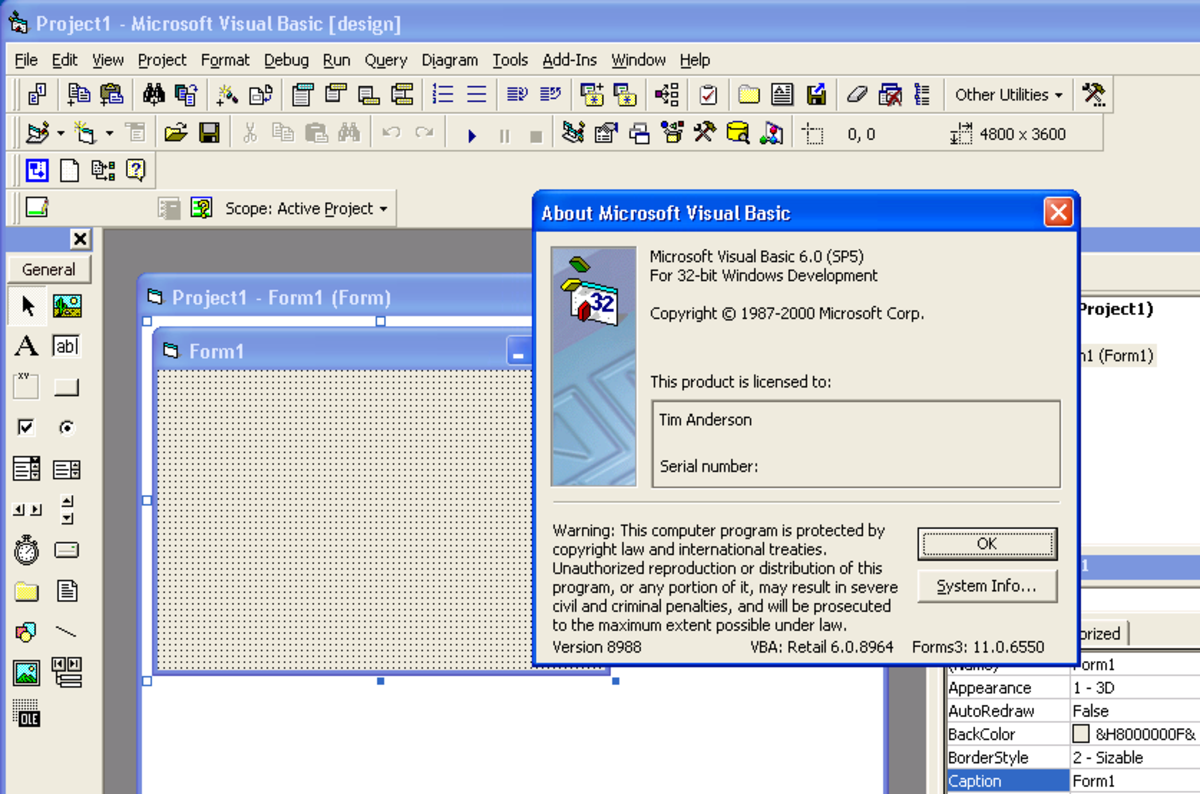
\includegraphics[width=\linewidth]{vb6.png}
    \caption{Voorbeeldweergave van de Visual Basic IDE \autocite{Speed2020}}
    \label{fig:vb6ide}
\end{figure}

LanReview werd gebouwd in Visual Basic (VB). Dit is een event-gedreven programmeertaal en omgeving van Microsoft waarmee programmeurs code kunnen aanpassen door drag-en-drop van objecten en door wijziging van hun gedrag en uiterlijk. VB komt van de BASIC programmeertaal. Het is een RAD (Rapid Application development) platform. Het werd voornamelijk gebruikt voor prototyping en als front-end voor databases. De laatste versie, Visual Basic 6.0, stamt van 1999.

Het grote voordeel is snelheid van ontwikkeling. Er zijn ook een aantal nadelen:
Het had veel geheugen nodig en was niet geschikt voor programma's die veel proceskracht nodig hadden, zoals games. Het is ook beperkt tot het Microsoft besturingssysteem.

\autocite{Rouse2019}

\subsubsection{Geschiedenis}

\begin{itemize}
    \item \textbf{1964}: BASIC geformuleerd door John Kemenu en Thomas Kurtz.
    \item \textbf{1987}: architect/programmeur Alan Cooper bedenkt voorloper van VB genaamd Tripod.
    \item \textbf{1988}: Bill Gates koopt de rechten voor Tripod.
    \item \textbf{1991}: Visual Basic 1.0 geïntroduceerd.
    \item \textbf{1998}: Visual Basic 6.0 geïntroduceerd.
    \item \textbf{2002}: .NET framework.
    \item \textbf{2008}: Einde extended support voor Visual Basic 6.0.
\end{itemize} \autocite{Grigonis2014}

\subsubsection{Vandaag}

Uitvoering van VB applicaties blijft ondersteund op moderne Windows versies. Het maken van nieuwe echter niet \autocite{MicrosoftDocs2018}. Niettegenstaande heeft men manieren gevonden om alsnog te installeren. \autocite{Brust2015}

Er is nog een kleine maar vocale groep aanhangers van VB. Dit komt omdat ze de officiële opvolger, Visual Basic .NET, niet waardig vonden voornamelijk omdat de afhankelijkheid van .NET een extra abstractielaag was. Voorbeelden hiervan zijn: % TODO: David Platt bron?
\begin{itemize}
    \item Visual Basic behoud blijft hoog. Opvallend aanhoudend succes voor een `dode` tool. \autocite{ISpliter2014}.
    \item Er werd een petitie gemaakt voor verdere ontwikkeling van VB. \autocite{2005}
    \item Er worden nog steeds applicaties mee ontwikkeld \autocite{Ippolito2018}.
\end{itemize}

\subsection{LanReview werking}

% TODO: afbeelding 1

\begin{figure}[h!]
    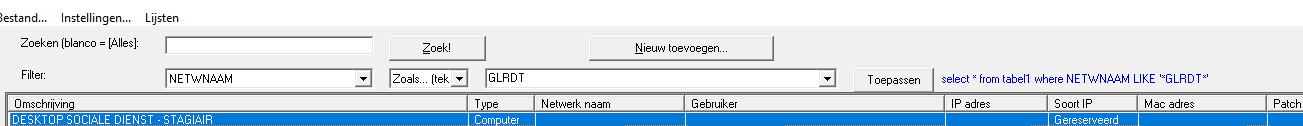
\includegraphics[width=\linewidth]{lanreview-overzicht-redacted.png}
    \caption{LanReview algemeen/filterbaar overzicht}
    \label{fig:lr-hoofd}
\end{figure}

LanReview houdt zijn informatie over assets in het domein bij in een Access databank. Deze informatie werd origineel geëxporteerd uit SCCM.
De applicatie heeft twee views: de primaire view is een filterbaar overzicht van devices. voor elke entry kan een meer gedetailleerde view opgeroepen waar alle datavelden te zien zijn.
Aan de hand van de filter functionaliteit worden SQL achtige queries gebouwd die dan uitgevoerd worden op de Acces databank.

LanReview is een belangrijke tool van de Helpdesk en wordt dagelijks gebruikt.

Vaak voorkomende use cases:
\begin{itemize}
    \item De pc overnemen van iemand in nood. Het is een startpunt voor remote management.
    \item Rapportage. Er kunnen voorgebouwde query's uitgevoerd worden op de data waarvan de resultaten onder andere naar Excel geëxporteerd kunnen worden.
    \item Filteren van de dataset. Bijvoorbeeld een overzicht van alle laptops van een belaad model tonen die nog steeds met Windows 7 werken.
    \item End of life beheer. Via markeringen is duidelijk of een device nog niet gebruikt wordt, in gebruik is of niet meer gebruikt wordt/in storage is.
\end{itemize}

% TODO: uiteg datavelden

\begin{figure}[h!]
    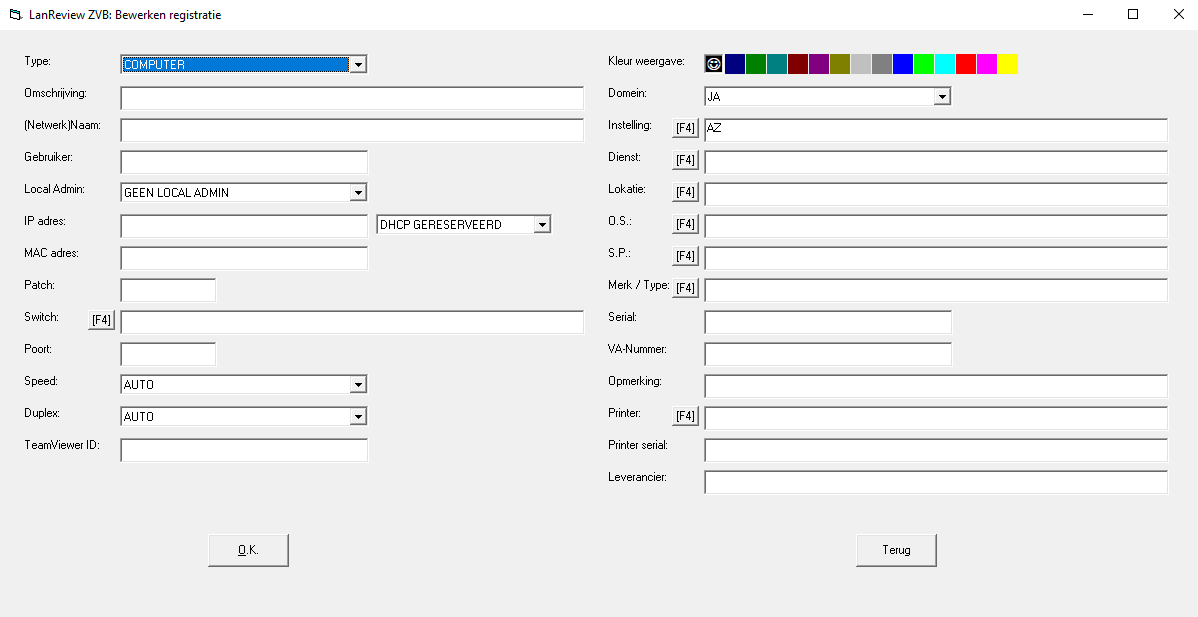
\includegraphics[width=\linewidth]{lanreview-detail-redacted.png}
    \caption{LanReview detailoverzicht}
    \label{fig:lr-detail}
\end{figure}

\section{Low Code}

\subsection{Basics}

De POC zal gebouwd worden met een low-code platform. Cloud services maken hier een deel van uit. Moderne low-code platformen zijn gecategoriseerd als PaaS (Platform as a Service). In geval van IaaS (infrastructure as a service) leeft de volledige infrastructuur in de cloud. PaaS kan gezien worden als een extra laag gebouwd bovenop IaaS waarmee applicatieontwikkelaars software kunnen programmeren in de cloud om later aan te kunnen bieden als SaaS (Software as a Service). Het is een tussenlaag gefocust op programmeurs. \autocite{Nucleus2017}

Definiëren van wat low-code zoal inhoud kan best begonnen worden met een formele definitie:\\
\textit{`It is an application platform that supports rapidapplication development, one-step deployment, execution and management using declarative,high-level programming abstractions, such as model-driven and metadata-based programminglanguages. They support the development of user interfaces, business logic and data services,and improve productivity at the expense of portability across vendors, as compared withconventional application platforms.`} \autocite{Vincent2019}

De bedoeling van low-code is om applicaties sneller te kunnen maken en ontwikkeling voor een grotere groep toegankelijk te maken. Typisch gezien wordt er een WYSIWYG (What You See Is What You Get) interface gebruikt waarin visuele componenten geconfigureerd worden via drag-and-drop. Vaak is er ondersteuning om aangepaste toe te voegen indien het platform bepaalde functionaliteit out of the box niet ondersteund. \autocite{Kissflow2018}

Low code is een software ontwikkelingsaanpak dat snellere oplevering van applicaties mogelijk maakt met minimaal manueel coderen. Dit werkt met visueel modeling in een grafische user interface om applicaties op te zetten en configureren. Hiermee slaat de ontwikkelaar de infrastructuur en her-implementatie van patronen die hun werk vertraagd en kunnen ze focussen op de unieke 10\% van een applicatie. \autocite{Revell2020}

Kissflow legt in zijn omschrijving nadruk op een grotere toegankelijkheid en Outsystems focust meer op het kunnen vermijden van herhalend werk.

Een low-code platform bestaat typisch uit volgende delen:
\begin{itemize}
    \item Een visuele IDE (Integrated Development Environment).
    \item Connectoren naar back-ends of services.
    \item App Lifecycle Management. Hiermee bedoelt geautomatiseerde tools voor build, debug, en deploy. Ook beheer van de app tijdens test, staging en productie.
\end{itemize} \autocite{Revell2020}

\subsubsection{low-code VS no-code}

Een no-code platform is een gespecialiseerde versie van een low-code platform waar men manuele aanpassingen zoveel mogelijk wil vermijden, al dan niet door het pre-builden van de nodige visuele componenten.

\textcite{Bloomberg2017} nuanceert de verschillen door te focussen op de bedoelde gebruiker:
\begin{itemize}
    \item low-code: Volgende generatie applicatie ontwikkeling dat het werk van professionele ontwikkelaars versneld en stroomlijnt.
    \item no-code: Self-service applicatie assembly voor business users die citizen developers worden.
\end{itemize}

\subsubsection{low-code development VS traditional software development}

% TODO: extra uitleg

\begin{landscape}
\begin{table}[]
    \begin{tabular}{@{}lll@{}}
        \toprule
        & \textbf{Traditional} & \textbf{Low Code} \\ \midrule
        1 & requirements bepalen & requirements bepalen \\
        2 & architectuur plannen & derde partij API's selecteren \\
        3 & selectie van back-end framework, bibliotheken, data-stores en API's & app workflow, data models en user interface tekenen in de visuele IDE \\
        4 & selectie van front-end framework & API's verbinden \\
        5 & keuze van deployment stack, opzetten van CI (Continuous Integration) en operatieplan creeren & indien nodig handgeschreven code toevoegen aan front-end of aanpassing van automatisch gegenereerde SQL queries \\
        6 & wireframes en prototypes maken & gebruikersacceptatietests \\
        7 & ui coderen in gekozen Javascript framework & deployment naar productie, hierna updates eenvoudig doorduwen \\
        8 & falende tests schrijven &  \\
        9 & modellen definieeren en koppelen aan data stores &  \\
        10 & business logic definieeren en coderen &  \\
        11 & views maken om JSON data te voorzien/ontvangen van en naar de front-end &  \\
        12 & implementeren van workflows &  \\
        13 & integreren van derde partij API's via gepubliceerde interface of support bibliotheek &  \\
        14 & herhalen tot tests slagen &  \\
        15 & testen voor security, performance, kwaliteit en gebruikersacceptatie &  \\
        16 & deploy, patch, monitor en updat tot levenseinde van de app &  \\ \bottomrule
    \end{tabular}
\end{table} \autocite{Revell2020}
\end{landscape} 

\subsubsection{Citizen developers}

De survey uitgevoerd door \textcite{McKendrick2017} geeft de volgende definitie:\\
\textit{`we define citizen developers as business users, not part of IT departments or contracted IT services, who build and use their own scripts, programs, algorithms, or interfaces designed to perform business functions or support business processes.`}

Er zijn enkele interessante statistieken uit voortgekomen:
\begin{itemize}
    \item Snelheid van applicatie delivery en delen van data/analytics worden aanzien als zwakke gebieden van IT support.
    \item 76\% van de respondenten zegt dat op z'n minst een deel van de gebruikte applicaties buiten het IT departement komen.
    \item 45\% van citizen development activiteiten worden tijdens de werkuren gedaan, de grootste motivatie hiervoor (42\%) is omdat het IT departement te traag is.
    \item In slechts 17\% van de gevallen duurt ontwikkeling van een citizen developer applicatie langer dan drie maand.
\end{itemize}

\subsubsection{Mythes}

Er bestaan enkele mythes rondom low-code:
\begin{itemize}
    \item Minder geschikt voor professionele gebruikers dan voor citizen developers \\
    $\rightarrow$ In praktijk wordt low-code vaker gebruikt door professionele ontwikkelaars.
    \item De nood om te programmeren wordt geëlimineerd \\
    $\rightarrow$ Het is vaak mogelijk om eenvoudigere applicaties te bouwen zonder code. Een typische business applicatie zal echter extra programmatie nodig hebben voor integratie met andere applicaties en databases, ook om aangepaste algoritmen te kunnen gebruiken. Deze use cases worden als extensies, externe programmatie of als scripts toegevoegd.
    \item low-code betekend kleine schaal \\
    $\rightarrow$ Er zijn genoeg praktijkvoorbeelden die dit tegenspreken. Neem bijvoorbeeld Sapphire HMS. \autocite{Bashar2017}
\end{itemize} \autocite{Richardson2016}

\subsection{Geschiedenis}

De oorsprong van low-code kan best bekeken worden vanuit het perspectief van de verranderingen in complexiteit en bruikbaarheid van programmeertalen doorheen de jaren. Er zijn enkele grote sprongen waarneembaar:
\begin{itemize}
    \item \textbf{Fortran}: niet intuïtief, nuttig voor wetenschappelijke en numerieke computing.
    \item \textbf{Cobol}: Focus buiten wetenschappers of wiskundigen. Syntax staat dichter bij Engels. Het hielp bij het vinden van oplossingen naar business taken.
    \item \textbf{C}: Geschreven met Engelse syntax. Bruikbaar in een grote variatie aan applicaties.
    \item \textbf{Internet}: Kwam door het internet en een groeiende populariteit van webapplicaties. Men is kleinere en eenvoudigere scripts beginnen gebruiken in plaats van complexe programmeertalen. Er was een focus op functie. Applicaties moeten aan een snellere pas ontwikkeld kunnen worden en talen moeten eenvoudig genoeg zijn om dit te ondersteunen.\\
    Een voorganger van low-code dat ook uit het internet is voortgekomen is het content management systeem. Wordpress is een bekend voorbeeld. Er zijn gelijkenissen in ideologie: het laat toe om de inhoud van een website aan te passen met een minimale hoeveelheid programmeren. Er worden modules gebruikt voor vaak voorkomende requirements. \autocite{Kissflow2018}
\end{itemize} \autocite{Kissflow2018a}

De ideologie achter low-code bestaat al een lange tijd. Er zijn cyclussen waar te nemen waarin de populariteit piekte. Een iteratie van 10 jaar geleden is 4gl (Fourth Generation Language). Een iteratie van 20 jaar geleden is RAD (Rapid Application Development). % TODO: welke bron?

Visuele en declaratieve development tools bestaan al decennia maar elke iteratie zijn er minder technische skills nodig om complexere business apps te kunnen maken die ook kunnen omgaan met moderne scenario's. Moderne low-code platformen overstijgen de limieten van op een aantal manieren: \\
\textbf{Ze zijn meer `open`.} Vaak worden platform API's en adapters ondersteund. Soms is mogelijk om Java of .NET code te genereren als maatregel tegen vendor lock-in. Sommige platformen gebruiken zelf open source development frameworks zoals AngularJS, Apache Cordova en Bootstrap.\\
\textbf{De platformen zelf zijn `completer`.} De vorige generaties waren eerder tools. Moderne low-code platformen ondersteunen de volledige applicatie levenscyclus.\\
\textbf{Betere integratiemogelijkheden.} De meeste low-code platformen laten laten toegang tot tot externe data toe. Vaak zijn er API's voor integratie mer externe applicatie modules. 

\autocite{Richardson2016}

\subsection{Nood / Voordelen}

\begin{figure}[h!]
    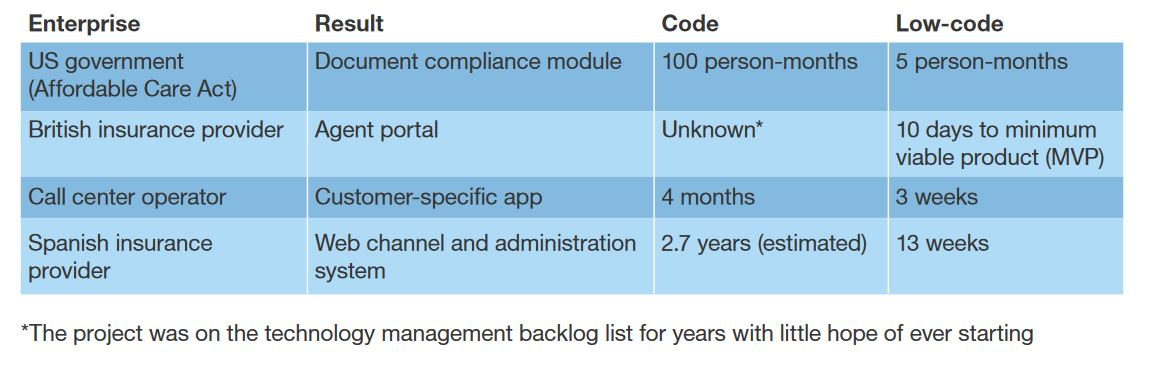
\includegraphics[width=\linewidth]{lowcode-time.JPG}
    \caption{Vergelijking van doorlooptijd \autocite{Richardson2016}}
    \label{fig:tijdverschil}
\end{figure}

Het verkooppunt van low-code is hogere snelheid van applicatieontwikkeling. Naast deze snelheid zijn er nog andere voordelen:
\begin{itemize}
    \item Betere collaboratie tussen business en IT: Business shareholders zien hun visie sneller vorm nemen en kunnen rappe aanpassingen doorvoeren. Business regels zijn geïntegreerd in het bouwen van de applicatie.
    \item Focus op functionaliteit: Er wordt geen tijd verspild met schrijven van herhalende code.
    \item Transparante deployment: Er zijn geen aanpassingen meer nodig om verschillende architecturen te kunnen ondersteunen.
    \item Lange termijn gebruik: Apps zijn eenvoudig aan te passen.
    \item Enkele code base: Minder ruimte voor fouten en de code base wordt ook niet vervuild met tijd.
\end{itemize} \autocite{Schetsen2016}

Markt leidende platformen hebben de volgende eigenschappen:
\begin{itemize}
    \item Eenvoudige visuele configuratie
    \item Veel integratie opties.
    \item Mobile compatibel.
    \item Schaalbaar.
    \item Support over de volledige app levenscyclus.
\end{itemize} \autocite{Kissflow2018}

Het perspectief van de klant, welke waardepropositie er is. Dit is duidelijker als er eerst naar de omgeving gekeken wordt. Bedrijven moeten steeds meer kunnen omgaan met disruptieve innovatie en wijzigend klantgedrag. De vraag naar applicaties is vaak groter dan wat geleverd kan worden. Er zijn strategieën om hier mee om te proberen gaan zoals outsourcing, hackathons of voorgebouwde softwareoplossingen. Low code is een nieuwe manier om er mee om te kunnen gaan. De waardepropositie voor de business en het tech management is:
\begin{itemize}
    \item Apps visueel configureren in plaats van manueel te coderen. Ontwikkeling kan zo mogelijk met een factor 5 tot 10 versneld worden.
    \item Echte requirements en zo echte waarden vinden. Met low-code kunnen snel minimum viable products gebouwd worden om klantenideeën te toetsen.
    \item Live-trial van business ideeën tegen lage of onbestaande kost. Ideen kunnen snel omgezet worden in een werkend prototype dat gedeployed en getest kan worden op de markt.
    \item Werkende prototypes kunnen in vijf minuten omgezet worden in productie apps. Het komt niet voor dat een app opnieuw gebouwd moet worden om een hoger volume of hogere diversiteit van gebruikers aan te kunnen.
    \item Meer development talent mogelijk. Developers zonder formele achtergrond kunnen door het visuele aspect nu ook business applicaties bouwen.
\end{itemize} \autocite{Richardson2016}

\subsubsection{Digitale transformatie}

Digitale transformatie is het proces van het gebruik van digitale technologie om nieuwe - of bestaande - business processen, cultuur en klantenexperience te maken als antwoord op veranderende business en markt requirements. Het is kortweg opnieuw bedenken van business in het digitale tijdperk. \autocite{Salesforce}
Digitale transformatie wordt steeds belangrijker als arena waarin business een voordeel kan krijgen op de competitie. Low-code wordt hierbij aanzien als een krachtig wapen in dit proces.

\subsection{Kritiek / Nadelen}

Er zijn een aantal valkuilen waar rekening mee gehouden moeten worden bij de keuze van een platform. De inzetting kan falen en het gewenste resultaat kan uitblijven als de klant geen concreet plan heeft over hoe low-code in te werken in zijn portfolio. Het is ook aangeraden om op te passen indien er een kleinere vendor gekozen wordt. Het is een veranderende markt en deze hebben een lagere stabiliteit. \autocite{Richardson2016}

Een mening is dat de business kant zijn mentaliteit ten opzicht van IT moet aanpassen. Al decennia probeert met de nood van programmeren terug te drijven en in functie hiervan worden tools gemaakt. Bedrijven zijn hiertoe aangetrokken om kosten te kunnen besparen. Maar de achterliggende kennis blijft nodig, vooral als er iets fout gaat. Niet alles kan visueel gedaan worden. Development talent blijft dus nog nodig. De aanpassing in mindset die gevraagd wordt is dat business het feit aanvaard dat software ontwikkeling duur en moeilijk is en dat er geen schortcuts voor zijn. \autocite{Reselman2018}

Er kan gesteld worden dan niet elk low-code platform daadwerkelijk 'low-code' is en dat men hiervoor moet oppassen:
\begin{itemize}
    \item \textbf{NIET} low-code: Het platform genereert statisch code en verstopt deze effectief voor de gebruiker. De code is niet flexibel en schaalt niet. Dit staat digitale transformatie in de weg en verhoogt technical debt in plaats van dit te verlagen.
    \item \textbf{WEL} low-code: Het platform is flexibel en schaalbaar. De volledige levenscyclus van de app moet ondersteund worden. Achterliggend wordt een model gedreven architectuur gehanteerd. De flexibiliteit komt doordat de model componenten geabstraheerd worden naar XML. De applicatie kan ook makkelijker gewijzigd worden en is eenvoudig schaalbaar.
\end{itemize} \autocite{Shiah2018}

\subsubsection{Shadow IT}

Gebruik van no-code tools in de handen van citizen developers kan mogelijk leiden tot shadow IT. Dit komt voor wanneer de IT organisatie te traag en proces-gebonden is om snel genoeg te kunnen reageren op de noden van business en business users buiten IT gaan om zelf een app bouwen. Zonder overzicht en coördinatie kunnen security kwetsbaarheden en compliance overtredingen verspreiden. Deze apps kunnen ook redundant en van lage kwaliteit zijn. \autocite{Bloomberg2017}

\subsection{Markt en Evolutie}
\label{sec:markt-en-evolutie}

\begin{figure}[h!]
    \centering
    \begin{subfigure}[b]{0.4\linewidth}
        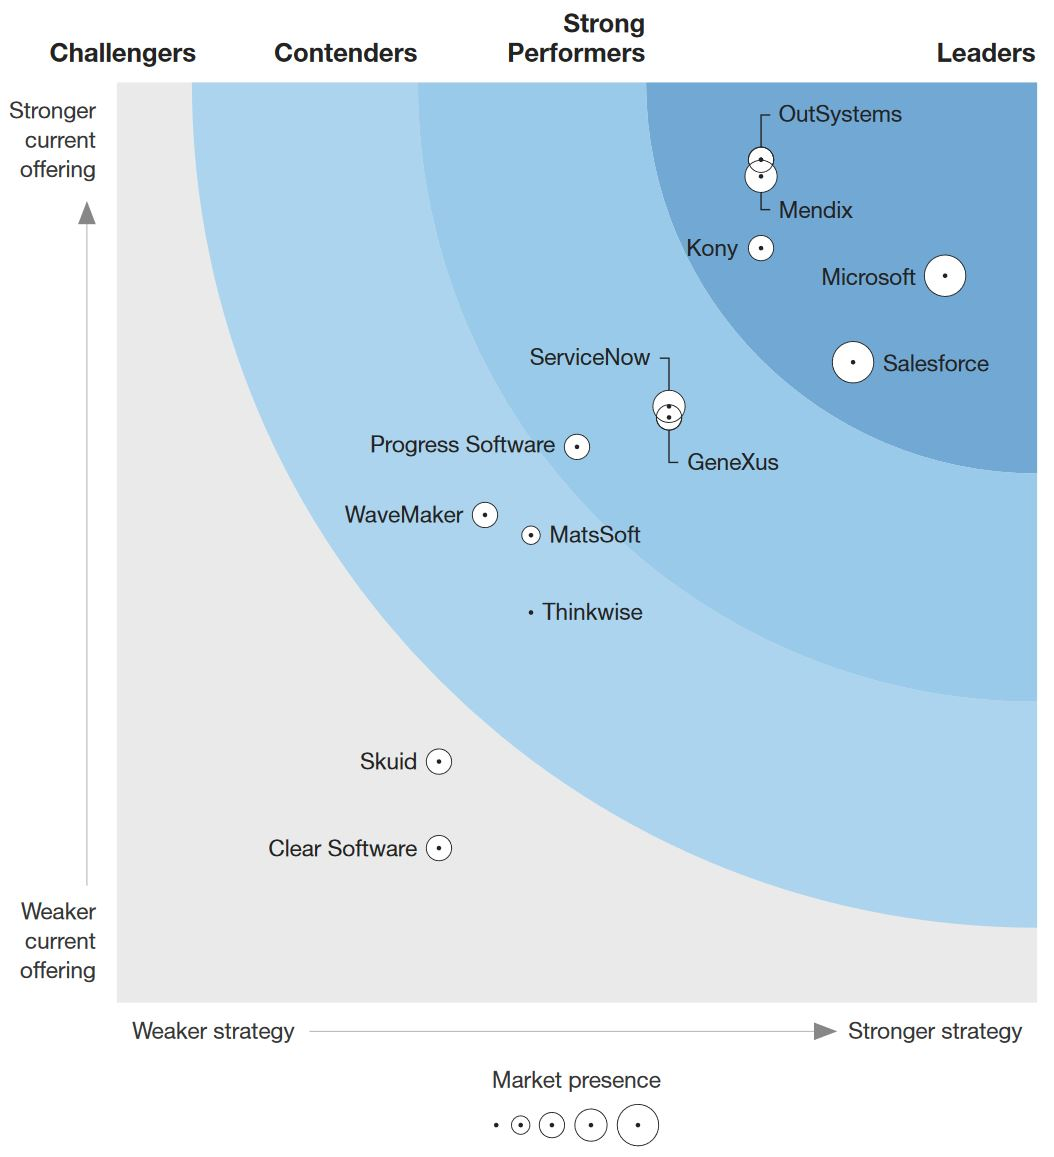
\includegraphics[width=\linewidth]{forrester-wave.JPG}
        \caption{Forrester Wave \autocite{Rymer2019}}
    \end{subfigure}
    \begin{subfigure}[b]{0.4\linewidth}
        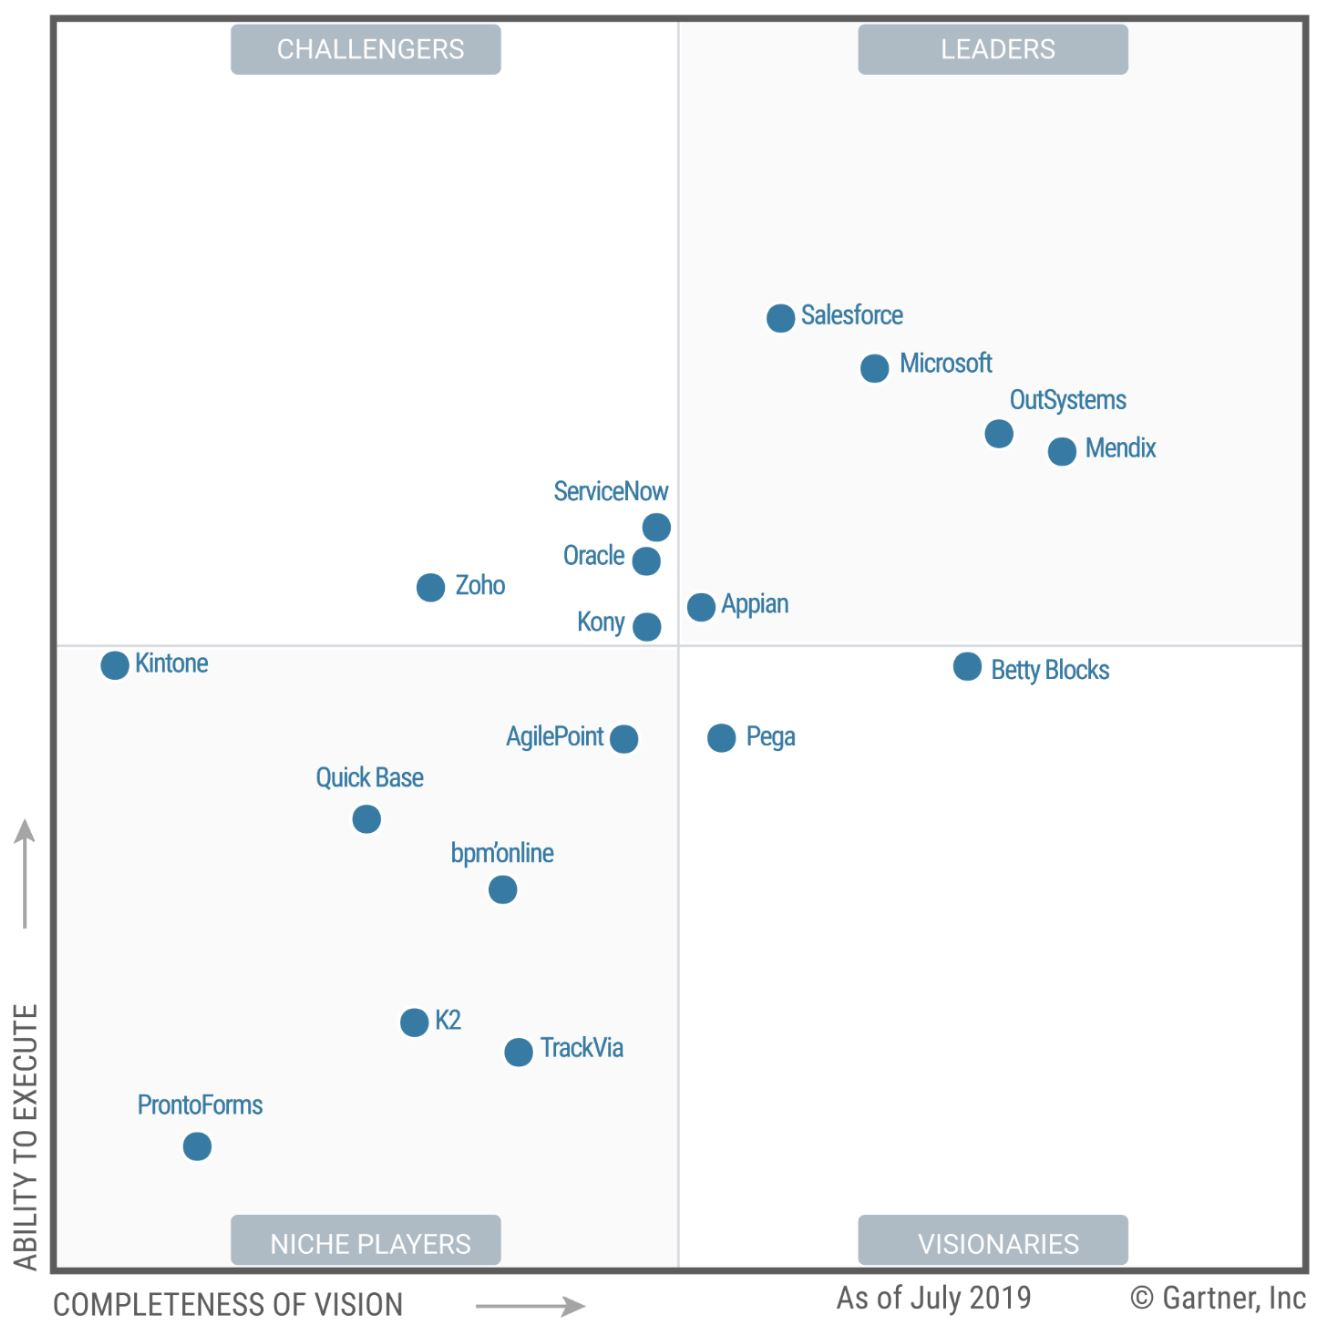
\includegraphics[width=\linewidth]{gartner-quadrant.JPG}
        \caption{Gartner Magic Quadrant \autocite{Vincent2019}}
    \end{subfigure}
    % \caption{overkoepelende caption}
    \label{fig:quadwave}
\end{figure}

Het business model van low code platformen is anders dan dat van traditionele platformen zoals Java of .NET. Er wordt uitgegaan van geleverde business waarde in plaats van beloofde. Zo zijn veel platformen gratis of tegen lage kost toegankelijk. Inkomst wordt gegenereerd uit benoemde gebruikers, gedeployde apps en nodige capaciteit. \autocite{Richardson2016}

Wat betreft marktsegmentatie heeft er zicht op relatief korte tijd veel evolutie voorgedaan. Er kunnen drie grote stappen onderscheiden worden:
\begin{enumerate}
    \item 5 marktsegmenten waarvan de grootste general purpose is. Het doel is grote variatie aan web en mobiele applicaties kunnen bouwen. Declaratieve tooling gebruikt met aandacht voor creatie, integratie, deployment life-cycle management en distributie van applicaties. Hiernaast waren ook nog segmenten voor process, database, request-handling en mobiele apps.
    \item Samensmelting naar general purpose % TODO: bron
    \item Splitsing om te focussen op gebruiker. Business user of professionele ontwikkelaars. % TODO: bron
\end{enumerate}

Er worden een aantal marktontwikkelingen verwacht:
\begin{itemize}
    \item \textbf{Consolidatie}. Grote verkopers zullen low-code platformen overnemen.
    \item \textbf{Marktsegment veranderingen}. Low code for mobile verdwijnt en low-code for process groeit naar general purpose segment.
    \item De volgende innovatie zal \textbf{ondersteuning voor IoT} zijn.
\end{itemize} \autocite{Richardson2016}

\textcite{Rymer2019} identificeert 5 marktleiders. Opvallend is dat Microsoft in een korte periode naar een leidingspositie is gesprongen. De bevindingen van \textcite{Richardson2016} sluiten hierbij aan.

\begin{table}[]
    \begin{tabular}{|l|l|l|l|l|l|}
        \hline
        \textbf{Forrester} & Salesforce & Microsoft & Mendix     & Outsystems & Kony   \\ \hline
        \textbf{Gartner}   & Salesforce & Microsoft & Outsystems & Mendix     & Appian \\ \hline
    \end{tabular}
    \caption{Overzicht van de marktleiders}
    \label{table:leiders}
\end{table}

Prospecten voor de komende vijf jaar:
\begin{itemize}
    \item Tegen 2024 zal drie vierde van grot enterprises ten minste vier low code development platformen gerbruiken voor zowel IT app development en citizen development initiatieven.
    \item tegen 2024 zal low-code applicatie development verantwoordelijk zijn voor 65\% van totale applicatie ontwikkeling activiteit.
\end{itemize} \autocite{Vincent2019}

De verschuiving van traditionele naar low-code software ontwikkeling is terug te vinden in huidige jobaanbiedingen\footnote{\url{https://stagebank-hbo-ict.irp.nl/internships/12543/}}\footnote{\url{https://stagebank-hbo-ict.irp.nl/internships/12378/}}.

Er wordt verwacht dat de low-code markt tegen 2022 21 biljoen dollar waard zal zijn. Er wordt ook voorspeld dat de jaarlijkse groei van 50\% zich verder zal zetten. \autocite{Rymer2018}

\begin{figure}[h!]
    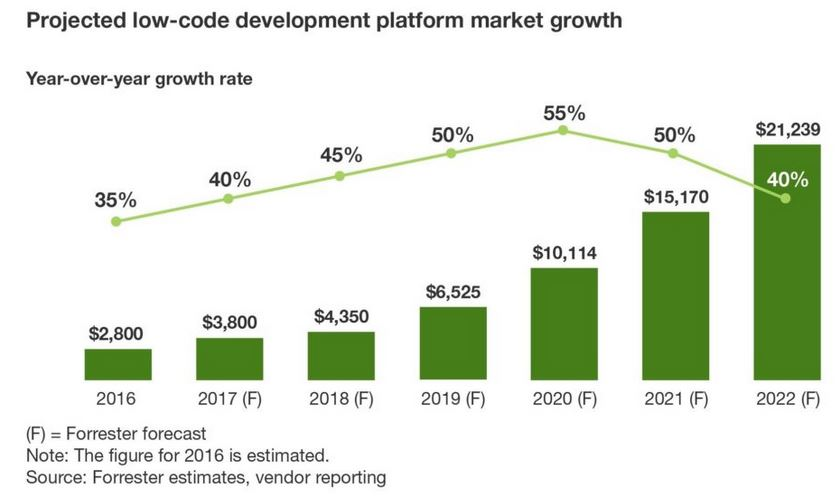
\includegraphics[width=\linewidth]{forrester-markt-evolutie.JPG}
    \caption{Forrester voorspelde markt evolutie \autocite{Rymer2018}}
    \label{fig:marktevolutie}
\end{figure}

\subsection{Voorgaand onderzoek}

Er is al redelijk wat praktisch onderzoek gevoerd die het potentieel van low-code illustreert maar het grootste succesverhaal is dat van Sapphire HMS. Dit is een low-code applicatie binnen gezondheidszorg. Koeweit had nood aan een nieuw ziekenhuis managementsysteem. Na initieel falen om iets manueel te bouwen werd gekeken naar low-code platformen en was het mogelijk om de eerste implementatie na 6 maanden in gebruik te nemen. \autocite{Bashar2017}

\subsubsection{Proof of Concepts}

Er werd onderzoek gedaan naar de mogelijke meerwaarde van low-code in een KMO omgeving. Uit vier marktleidende platformen werd Outsystems gekozen. Er werden POC's voor vaak voorkomende scenario's mee opgesteld. De bouw we snel, eenvoudig en er waren geen obstructies. De nodige investering van tijd, geld en kennis was beperkt \autocite{Devloo2018}.

Microsoft Power Apps werd gebruikt om enkele administratieve bedrijfsprocessen van verhuisbedrijf De Borger te optimaliseren. Het resultaat werd effectief in gebruik genomen de tijdswinst sinds implementatie werd berekend en significant bevonden. De prijs was aanvaardbaar. Er was slechts 5 euro per maand nodig om een aangepaste connector te kunnen gebruiken. \autocite{Spriet2019}

In een ander geval werd Power Apps gebruikt om een mobiele reporting applicatie te maken voor gebruik in de bouwsector. Er werd ok gebruik gemaakt van Power Automate om afbeeldingen te verwerken en SharePoint om deze op te slaan. \autocite{Aho2018}

Binnen de gezondheidszorg werd er een case study gedaan naar hoe onderzoeksdata verzameld kon worden door gebruik van een low-code platform. Er werd voor Mendix gekozen. De veiligheid van het platform werd als goed bevonden, relevant privacywetten waren gerespecteerd en authenticatie werd ondersteund en was eenvoudig te implementeren. Er werd verhoogde productiviteit waargenomen. \autocite{Totterdale2018}

\subsubsection{Enquetes}

Er werd onderzocht of het mogelijk zou zijn om een EHR (electronic Health Records) systeem te bouwen met low-code om te gebruiken op nationaal niveau. Dit was naar aanleiding van het Akson planningsproject voor een nieuw EHR systeem in Noorwegen. Er werden kwalitatieve interviews afgenomen bij mensen met expertise in low-code en mensen met kennis van het Akson project. \autocite{Ness2019}

Low-code en traditionele softwareontwikkeling werden met elkaar vergeleken aan de hand van interviews met medewerkers bij een Fins software consultancy bedrijf. Er kon besloten worden dat zowel de medewerkers als de klanten oplossingen gebouwd met low-code verkozen. \autocite{Virta2018}

\section{Microsoft Power Platform: Power Apps}
\label{sec:power-platform}

\subsection{Wat?}

\begin{figure}[h!]
    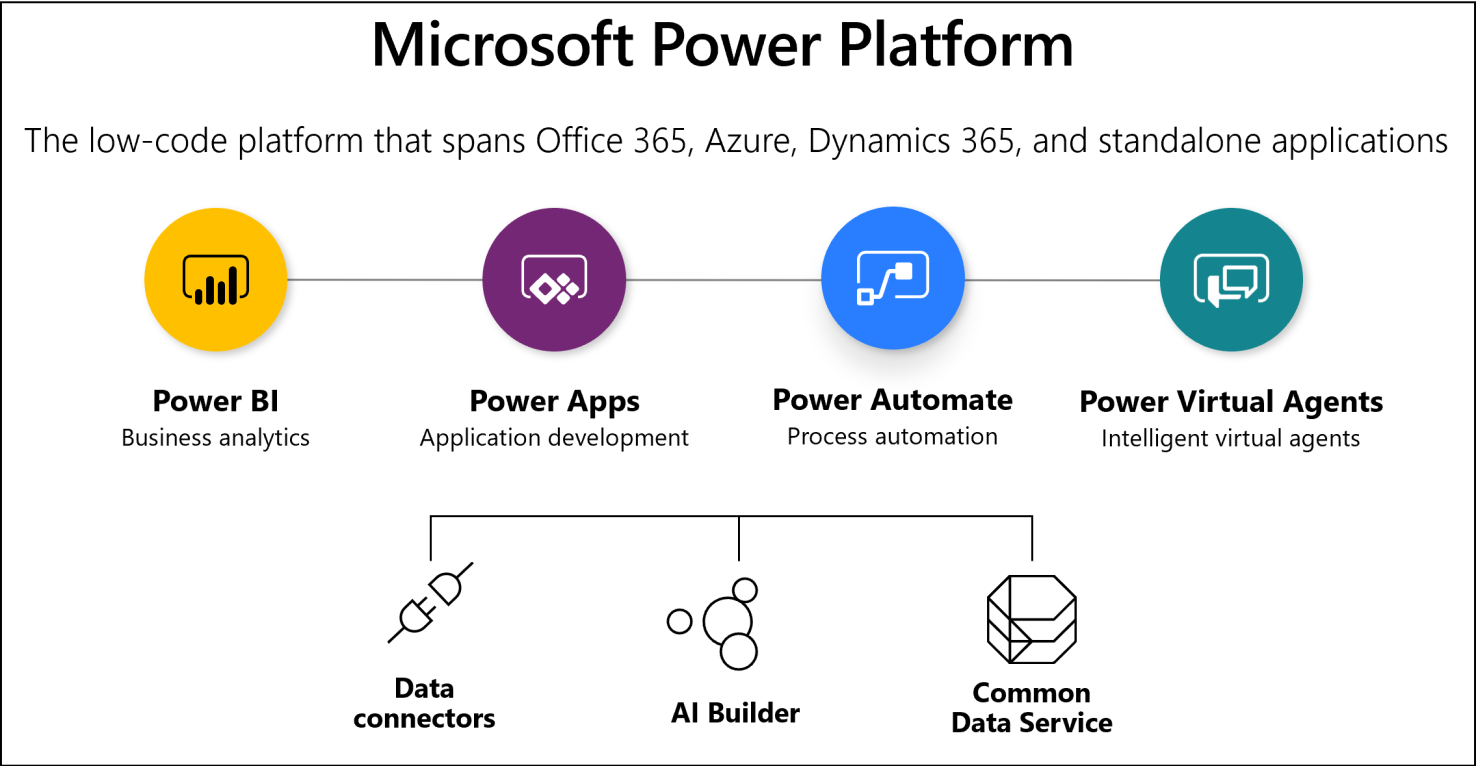
\includegraphics[width=\linewidth]{platform.png}
    \caption{Overzicht Microsoft Power Platform \autocite{MicrosoftDocs2019a}}
    \label{fig:mspowerplatform}
\end{figure}

Power Apps is een suite met apps, services en connectors. Het is een gegevensplatform die een snelle ontwikkelomgeving biedt om aangepaste apps te bouwen voor zakelijke behoeften. Men kan verbinden met zakelijke gegevens die zijn opgeslagen ofwel in het onderliggend gegevensplatform (Common Data Services), ofwel in de verschillende online en on-premises gegevensbronnen (SharePoint, Excel, Office 365, Dynamics 365, SQL Server enzovoort). De apps hebben een responsief ontwerp en kunnen zowel in een browser of op mobiele apparaten (telefoon of tablet) uitgevoerd worden. \autocite{MicrosoftDocs2019}

\subsection{Drie soorten apps}

\subsubsection{Canvas apps}

Populairste en meest toegankelijke variant. Er is een focus op het grafische. Zo worden de apps via een WYSIWYG (What You See Is What You Get) manier gebouwd. Daarmee is er volledige controle over de User Experience. Er is zowel tablet als mobile layout mogelijk. Men kan verder connecteren met meerdere data bronnen. Het resultaat zijn taak- en rol gebaseerde apps. \autocite{PragmaticWorks2019}

\subsubsection{Model Driven apps}

In tegenstelling tot Canvas apps begint men hier bij het data model. Deze data moet ook in de CDS leven. Het doel is meestal om complexe business processen te visualiseren. Het resultaat zijn dan ook end-to-end business applicaties. \autocite{PragmaticWorks2019}

\subsubsection{Portals}

Waar Canvas en Model apps naar binnen, naar internet business gebruikers gericht is, is Portals naar buiten gericht. Met portals kunnen extern gefocuste websites gebouwd worden waarmee gebruikers buiten de organisatie kunnen inloggen met een variëteit aan identiteiten, data in de Common Data Services kunnen bekijken of inhoud anoniem browsen. Er zijn zowel interne als externe gebruikers mogelijk. \autocite{MicrosoftDocs2020a}

\subsection{Belangrijke Onderdelen}

\subsubsection{Common Data Service}

Met de common data service kan data gebruikt door business applicaties opgeslagen en gemanaged worden. Data wordt opgeslagen binnen een set entiteiten. Een entiteit is een set van records om data op te slaan, zoals tables data opslaan in een database. Er zijn standaard entiteiten aanwezig voor typische scenario's, er kunnen ook aangepaste entiteiten gemaakt worden. Data wordt opgeslagen in de cloud. Er is ook logica en validatie mogelijk in de vorm van berekende velden, business regels, workflows en business process flows. Het 'common' aspect: De databronnen zijn gelinkt, als data in de ene bron aangepast wordt zal de relevante data in de andere bron automatisch aangepast worden. \autocite{MicrosoftDocs2019a}

\subsubsection{Connectors}

Data die een app nodig heeft is opgeslagen in een data bron, deze data naar de app brengen wordt gedaan door er een connectie voor te maken. Deze connectie heft een specifieke connector nodig om te kunnen praten met de data bron. Power Apps heeft connectors voor enerzijds populaire services en anderzijds on-premises data opslag. \\
Een connector kan in de app zelf dan ofwel tabellen of acties voorzien.

Een overzicht van de belangrijkste connectors:
\begin{itemize}
    \item Common Data Service
    \item Cloud storage: Voor elke grote provider. Bijvoorbeeld Google Drive of OneDrive.
    \item Excel: om excel data te kunnen tonen in de app. Requirements zijn dat de data geformatteerd moet worden als tabel en het bestand in de Cloud opgeslagen moet zijn.
    \item Office 365 (Outlook): Onder andere mogelijk om mails te tonen, versturen, beantwoorden of te deleten.
    \item Office 365 (Users): Toegang tot de gebruikersprofielen in de organisatie.
    \item Oracle DB
    \item Power BI
    \item SharePoint
    \item SQL Server
    \item Twitter
\end{itemize} \autocite{MicrosoftDocs2020b}

\textbf{On-premises data gateway}: Om on-premises data bronnen te kunnen gebruiken binnen een Power is moet een er een data gateway voor aanwezig zijn. Dit is een soort van brug tussen de on-premises data en de Microsoft cloud services die veilige data overdracht garandeert. \autocite{MicrosoftDocs2019b}

\subsubsection{Formules}

\begin{figure}[h!]
    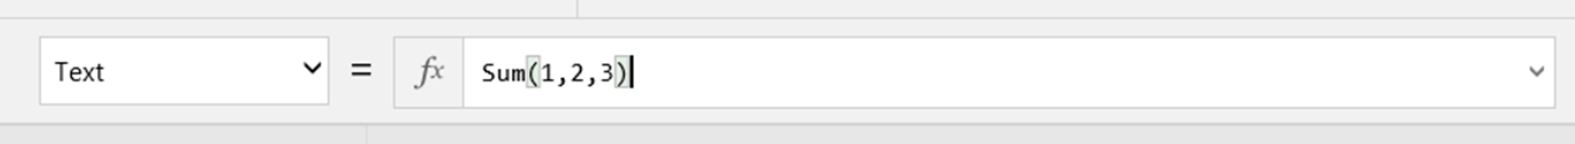
\includegraphics[width=\linewidth]{formula-bar.JPG}
    \caption{Overzicht van de formulebalk \autocite{MicrosoftDocs2019c}}
    \label{fig:msformulebalk}
\end{figure}

Logica en werken met gegevens is mogelijk met Excel-achtige expressies.\\
In Excel worden formules gebruikt om cellen te vullen of grafieken en tabellen te maken. In Power Apps worden vergelijkbare formules gebruikt om besturingselementen in plaats van cellen te configureren. Concreet ook om om te gaan met user input. De granulariteit is: een app bestaat uit UI controls $\rightarrow$ elke control heeft properties $\rightarrow$ per property kunnen formule(s) ingesteld worden. \autocite{MicrosoftDocs2019c}

\subsubsection{Overig}
\label{subsec:overig}

Nadat werk aan een app opgeslagen is moet deze gepubliceerd worden om bruikbaar te zijn voor ander leden van de organisatie.

Versiebeheer is beperkt aanwezig. Er kan eenvoudig teruggegaan worden naar eerder gepubliceerde versies van een app.

UI Tests zijn mogelijk met de Test Studio maar op moment van schrijven is dit nog experimenteel. Power Apps Test Studio is een low-code oplossing om tests te schrijven, organiseren en automatiseren voor canvas apps. In de Test Studio kunnen tests geschreven worden via Power Apps expressies of door gebruik van een recorder om app interactie op te slaan en expressies automatisch te genereren. De tests kunnen hierna teruggespeeld worden binnen de Test Studio om app functionaliteit te valideren. \\ 
Gebruikte concepten en terminologie komen overeen met gangbare testing frameworks zoals bijvoorbeeld JUnit voor Java. \\
Meer uitleg aan de hand van deze terminologie. 
\begin{itemize}
    \item \textbf{Test Cases}: Test cases bestaan uit een serie instructies of acties genaamd test stappen. Test cases worden utigevoerd om te controleren of apps of specifieke features in de app werken zoals verwacht. Deze test stappen zijn geschreven in de Power Apps expressie taal.
    \item \textbf{Test Suites}: Gebruikt om test cases samen te groeperen.
    \item \textbf{Test Assertions}: gebruikt om te valideren of het verwacht resultaat overeen komt met het verkregen resultaat. Evalueert naar true of false.
\end{itemize}
\autocite{MicrosoftDocs2019d}

Tot op heden werd is er nog geen IT Asset Management app gebouwd in Power Apps die als template terug te vinden is. Wel bestaat er een Asset checkout app. Dit staat er dicht genoeg bij. \autocite{Meganathan2019}

\subsection{IDE overzicht}

De onderdelen van Power Apps Studio uitgelicht volgens Figuur \ref{fig:pastudio}:
\begin{enumerate}
    \item Links: Hiërarchische view van de app screens en controls.
    \item Centraal: Huidige app scherm.
    \item Rechts: Geavanceerde layout en data bronnen.
    \item Property lijst voor geselecteerde control.
    \item Formulebalk.
    \item Ribbon.
\end{enumerate}

\begin{figure}[h!]
    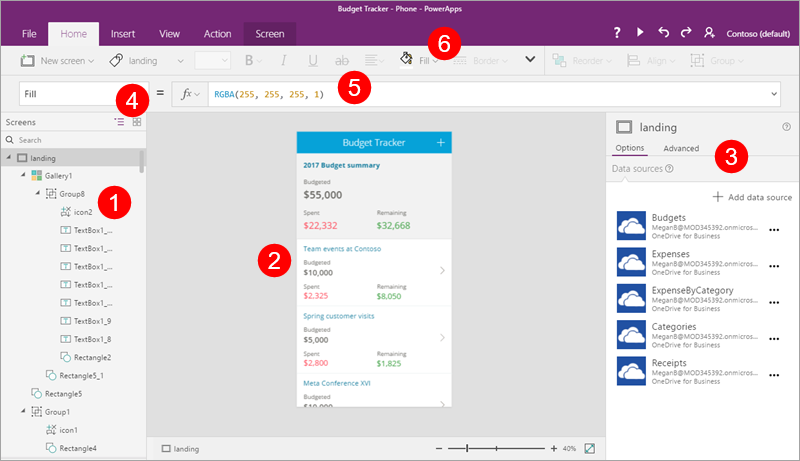
\includegraphics[width=\linewidth]{powerapps-studio.png}
    \caption{Overzicht van Power Apps Studio \autocite{MicrosoftDocs2017}}
    \label{fig:pastudio}
\end{figure}

\subsection{Recente Wijzigingen}

De Test studio valt hierbij (zie subsectie~\ref{subsec:overig}). % TODO: datum zetten

De AI Builder is in publieke preview sinds 10 juni 2019. Dit maakt het mogelijk om AI te gebruiken in Power Apps met minimale technische kennis.\\
Een voorbeeld van het typische verloop: Een AI model type kiezen $\rightarrow$ Data verbinden (uit CDS) $\rightarrow$ AI model aanpassen naar noden (data filteren, scheduling) $\rightarrow$ AI model trainen (gebeurt automatisch) $\rightarrow$ De inzichten van het AI model gebruiken doorheen het Power Platform.\\
Wat AI modellen betreft zijn er enkele keuzes: enerzijds kan er aan aangepast model gebruikt gemaakt worden (voorspelling, form processing, object detectie, text classificatie), anderzijds kan geopteerd worden voor een voorgebouwd. In dat geval is er geen data nodig, het is gebouwd (en getraind) door Microsoft. Mogelijke keuzes zijn: Business card lezer, sleutel zin extractor, taal detectie, text herkenning, gevoelsanalyse. \autocite{MicrosoftDocs2019e}

% TODO: iets over teams wijzigingen/integratie?

\subsection{Pricing, Licencing}

\begin{itemize}
    \item Power Apps voor Office 365.
    \item Plan 1
    \item Plan 2
    \item Power Apps for Dynamics.
\end{itemize} \autocite{Pohl2019}

Elke entry in de lijst heeft meer functionaliteit dan de voorgaande.\\
In Power Apps for office is het enkel mogelijk Canvas apps te maken. Het aantal connectors is beperkt. De on-premise connectors bijvoorbeeld zijn niet aanwezig.

\subsection{Uitbreidingsmogelijkheden}

Power Apps studio is bedoelt als no code omgeving gefocust op business gebruikers. Binnen deze ui is er geen optie om aangepaste code te gebruiken. De enige manier om dit mogelijk te maken is via Custom API's, Azure functions of Azure API apps \footnote{Volgens het antwoord van een Microsoft medewerker op het Power App forum: \url{https://powerusers.microsoft.com/t5/Power-Apps-Ideas/add-your-own-js-in-powerapps-or-call-external-js-file-easily/idi-p/869}}.\\
Praktisch gezien is dit mogelijk door een project te maken in Visual studio, een OpenAPI definitie te voorzien. Als deze app in de Azure cloud staan kan deze ook opgeroepen worden vanuit Power Apps \autocite{Jugo2019}

\section{Microsoft Power Platform: Power Automate}

Power automate is een service voor het maken van geautomatiseerde workflows tussen apps en services. Een flow kan gemaakt worden door stappen aaneen te schakelen. Per stap kan een actie of conditie ingesteld worden. In deze condities kunnen data operaties geconfigureerd worden, er zijn ook expressies mogelijk. Naast het zelf bouwen van een flow zijn er sjablonen aanwezig voor gangbare automatisatie cases. Flows kunnen gebruikt worden vanuit Power Apps. \autocite{MicrosoftDocs2019f}

Er zijn vijf soorten flows:
\begin{itemize}
    \item Geautomatiseerde flow: de flow wordt gestart vanuit een bepaalde trigger.
    \item Button flows: de flow wordt manueel gestart. Vaak wordt dit gebruikt vanop een mobiele device.
    \item Scheduled flows: De flow herhaald / op een schema uitvoeren.
    \item Approval flows
    \item UI flows: Een vorm van UI automatisatie, een optie indien er geen API of connector aanwezig is (bijvoorbeeld oudere toepassingen). Voor gebruik met Windows desktop en web applicaties. Momenteel nog in experimentele fase. Het kan gezien worden als een eenvoudige manier om een script te bouwen. De werking is dat de gebruiker een actie/set stappen opneemt, hier wordt dan een aanpasbare flow voor gegenereerd. \autocite{MPA2019}
\end{itemize}

\subsubsection{Beperkingen}

Er is geen aangepaste code of scripting ondersteund.
%%=============================================================================
%% Methodologie
%%=============================================================================

\chapter{\IfLanguageName{dutch}{Methodologie}{Methodology}}
\label{ch:methodologie}

%% TODO: Hoe ben je te werk gegaan? Verdeel je onderzoek in grote fasen, en
%% licht in elke fase toe welke stappen je gevolgd hebt. Verantwoord waarom je
%% op deze manier te werk gegaan bent. Je moet kunnen aantonen dat je de best
%% mogelijke manier toegepast hebt om een antwoord te vinden op de
%% onderzoeksvraag.

%\lipsum[21-25]

\section{Requirementsanalyse}


De bedoeling van deze analyse is uitvinden hoe goed Power Apps voldoet aan de requirements en mogelijks ontdekken of er een alternatief bestaat dat overwogen kan worden. Als PowerApps in de toekomst effectief gebruikt zal worden, voornamelijk door het IT en Helpdesk team, is het dan niet logisch om dit alternatief te laten conformeren aan de bedoelde eindgebruiker, zijnde professionele IT'ers? Dit idee zal mee spelen bij de besluitvorming.

\subsection{Functioneel VS Niet-functioneel}
De requirements werden opgesteld tijdens herhaalde gesprekken met zowel de co-promotor als een lid van het Helpdesk team dat de app effectief zou gaan gebruiken.
De resultaten zijn hieronder opgesplitst in functionele-\footnote{Functionele requirement: gewenst gedrag ven het systeem} en niet-functionele\footnote{Niet-functionele requirement: kwaliteitseis waaraan het systeem moet voldoen} requirements.

\begin{itemize}
    \item \textbf{Functionele requirements}
    \begin{itemize}
        \item Overzicht kunnen geven van belangrijkste info voor elk toestel in het netwerk.
        \item Rapporten kunnen genereren.
        \item PC's bedienen vanop afstand (Remote Desktop Protocol kunnen oproepen).
        \item Gerichte/basis taken kunnen automatiseren.
        \item Bruikbaar zijn buiten het domein.
        \item Mobiel bruikbaar zijn.
        \item Nieuwe types toestellen opnemen.
        \item Randapparatuur opnemen (= koppeling tussen toestellen).
        \item Revisie van elk dataveld per toesteltype.
        \item Data opslaan in SharePoint (cloud).
        \item Samenwerken met SCCM en/of synchroniseren met en data uit de SQL databank kunnen gebruiken.
        \item Barcodes kunnen scannen (toegang hebben tot camera, barcode functionaliteit ingebouwd).
        \item AI functionaliteit.
        \item Het Ping commando kunnen oproepen.
        \item Command line toegang hebben tot PC's.
        \item Intune integratie.
    \end{itemize}
    \item \textbf{Niet-functionele requirements}
    \begin{itemize}
        \item Prijs (geen prijsstijging voor de te implementeren case of voor het aantal gebruikers).
        \item Future proof\footnote{Hiermee bedoelt een algemene combinatie van achterliggende technologie, innovatie, consistentie en marktaanwezigheid} zijn.
        \item Diverse GUI verbeteringen (specifiek kleur markeringen, tabbladen)/robuust GUI ontwerp ondersteunen.
        \item Performant zijn (specifiek met grote hoeveelheden entries/rijen kunnen omgaan).
        \item Leercurve moet degelijk zijn (het gebruik ervan moet aanslaan na het onderzoek).
        \item Veiligheid (een must nodig omwille van gevoelige bedrijfsdata).
    \end{itemize}
\end{itemize}

\subsection{MoSCoW-methode}

De volgende stap is prioriteiten stellen onder de requirements. Hiervoor wordt de MoSCoW-methode\footnote{Must have: eis moet terugkomen in het eindresultaat, Should have: eis is zeer gewenst maar het product is bruikbaar zonder, Could have: eis komt aan bod als er genoeg tijd is, Won't have: komt niet aan bod, is voor de toekomst of een vervolgproject \autocite{Wikipedia2020}} gebruikt.

\begin{itemize}
    \item \textbf{\colorbox{green}{Must have}}
    \begin{itemize}
        \item Geen of beperkte meerprijs.
        \item Overzicht kunnen geven van belangrijkste info voor elk toestel in het netwerk.
        \item Rapporten kunnen genereren.
        \item PC's bedienen vanop afstand (Remote Desktop Protocol kunnen oproepen).
        \item Mobiel bruikbaar zijn.
        \item Future proof zijn.
        \item Performant zijn.
        \item Veiligheid.
        
    \end{itemize}
    \item \textbf{\colorbox{yellow}{Should have}}
    \begin{itemize}
        \item Gerichte/basis taken kunnen automatiseren.\\
        \textit{(Specifieke case: Een wekelijks rapport opstellen en rondmailen.)}
        \item Bruikbaar zijn buiten het domein.
        \item Nieuwe types toestellen opnemen.
        \item Randapparatuur opnemen.
        \item Revisie van elk dataveld per toesteltype.
        \item Data opslaan in SharePoint (cloud).
        \item Leercurve moet degelijk zijn.
    \end{itemize}
    \item \textbf{\colorbox{orange}{Could have (nice to have)}}
    \begin{itemize}
        \item Samenwerken met SCCM en/of synchroniseren met en data uit de SQL databank kunnen gebruiken.
        \item Diverse GUI verbeteringen/robuust GUI ontwerp ondersteunen.
        \item Barcodes kunnen scannen.
        \item AI functionaliteit.
        \item Het Ping commando kunnen oproepen.
    \end{itemize}
    \item \textbf{\colorbox{red}{Won't have}}
    \begin{itemize}
        \item Command line toegang hebben tot PC's.
        \item Intune integratie.
    \end{itemize}
\end{itemize}

\subsection{Long List}

Er zijn veel platformen om uit te kiezen\footnote{ 57 volgens een oplijsting van \href{https://www.trustradius.com/low-code-development}{TrustRadius}}. Degene hieronder opgelijst werden besproken in de Forrester Wave \autocite{Rymer2019} en het Gartner Magic Quadrant \autocite{Vincent2019}. De low-code markt kent een sterke groei en is zeer bewogen (zie sectie~\ref{sec:markt-en-evolutie}). Het eerste gekozen criteria om de lijst te filteren is bedoelt om hiermee om te gaan, het kan immers aangenomen worden dat een platform bestempelt door Gartner of Forrester als leider voldoende future proof is. Het andere gekozen criteria betreft het licentie model. Power Apps is opgenomen in het Office 365 licentie van AZ Glorieux, initieel gebruik ervan betekend geen dus geen meerprijs, een concurrent moet met andere woorden iets gelijkaardig kunnen aanbieden.

\begin{longtable}{llccc}
    \textbf{} & \textbf{} & \multicolumn{2}{c}{\textbf{Leider}} & \multicolumn{1}{l}{\textbf{}} \\
    \endfirsthead
    %
    \endhead
    %
    \textbf{Naam} & \textbf{Omschrijving} & \multicolumn{1}{l}{\textbf{Forrester}} & \multicolumn{1}{l}{\textbf{Gartner}} & \multicolumn{1}{l}{\textbf{Freemium}} \\
    AgilePoint &  &  &  &  \\
    Appian &  &  & x &  \\
    Betty Blocks &  &  &  &  \\
    bpm'online &  &  &  &  \\
    Clear Software &  &  &  &  \\
    GeneXus &  &  &  &  \\
    Kony &  & x &  & x \\
    K2 &  &  &  &  \\
    Kintone &  &  &  &  \\
    MatSoft &  &  &  & x \\
    Mendix &  & x & x & x \\
    Microsoft &  & x & x & (x) \\
    Outsystems &  & x & x & x \\
    Oracle &  &  &  &  \\
    Pega &  &  &  &  \\
    Progress Software &  &  &  &  \\
    ProntoForms &  &  &  &  \\
    Quick Base &  &  &  &  \\
    Salesforce &  & x & x &  \\
    ServiceNow &  &  &  & x \\
    Skuid &  &  &  &  \\
    Thinkwise &  &  &  &  \\
    TrackVia &  &  &  & x \\
    WaveMaker &  &  &  &  \\
    Zoho &  &  &  & x
\end{longtable}

Het resultaat is dat er van de leiders (zie tabel~\ref{table:leiders} voor een gefocuste weergave) slechts enkelen overblijven die in aanmerking komen.

\subsection{Short List}

% TODO: uitleg herleiden van requirements beter nuanceren?

Hier worden de overgebleven platformen in diepte met elkaar vergeleken Maar in plaats van elke requirement af te toetsen werden deze eerst herleid naar hun achterliggende begrippen (bijvoorbeeld: mobile ondersteuning, automatisatie functionaliteit, security, leercurve en dergelijke).

Gemaakte stellingen zijn afkomstig uit PCmagazine.com reviews van elk platform en zijn aangevuld met informatie uit de officiële documentatie per platvorm.
% TODO: pcMag veotnoot met overzicht reviews

\subsubsection{Microsoft}

Power Apps is deel van het Power platform (zie afbeelding~\ref{fig:mspowerplatform}). Het bestaat sinds 2016 en is daarmee het jongste platform in de vergelijking maar heeft een snelle ontwikkeling ondergaan en is op slechts enkele jaren tijd een marktleider geworden.

Werd diepgaand behandeld in de Stand van Zaken. (specifiek in sectie~\ref{sec:power-platform}). Een kort overzicht:

Gefocust op business users.
Apps worden gebouwd met de Power Apps Studio in de cloud. Deze omgeving is volledig grafisch, er is geen code editing. Uitbreidingang kunnen enkel ingevoegd worden via Azure Functions of Azure web apps en worden geschreven in .NET. Logica is gedeclareerd met een Excel-achtige formule taal. Er is een grote catalogus aan connectors naar externe service of data opslag. Verbinding maken met SharePoint data is eenvoudig met de Connector ervoor. Automatisatie is mogelijk via Power Automate waarin geautomatiseerde stromen van aaneengeschakelde acties geconfigureerd kunnen worden. AI werd recent geïntroduceerd, dit component heet AI Builder, naast zelf trainen van gangbare modellen biedt Microsoft enkele voorgetrainde aan. Nog in bèta is het testing framework genaamd UI Test Studio. Power Apps zijn gefocust op interne business gebruikers, voor externe bestaat er Portals. De leercurve is hoger dan van de concurrentie maar beschikbare documentatie en tutorials zijn talrijk en matuur. Performantie en vooral database performantie is lager dan van de concurrentie, er staat ook een limiet op het aantal rijen dat per keer opgehaald kan worden (500). Microsoft toont toewijding aan het platform door constante ontwikkeling maar sommige licentiewijzigingen zijn minder goed ontvangen.
% TODO: security aanvullen + bron met ()kritiek op) licentiewijziging

\begin{itemize}
    \item \textbf{Forrester}
    \begin{itemize}
        \item \textit{Positief:} Maturiteit bereikt, krachtige features en grote catalogus aan integratie adapters.
        \item \textit{Negatief:} Verwarrend product aanbod en licentiëring. Voor elk product van het Power platform is bijvoorbeeld een aparte licentie nodig.
    \end{itemize}
    \item \textbf{Gartner}
    \begin{itemize}
        \item \textit{Positief:} Eenvoudige drag-en-drop design tool en Exel-achtige  expressie taal. Snelle productie deployment mogelijk. Sterke toewijding aan LCAP markt getoond.
        \item \textit{Negatief:} Model apps niet altijd beste oplossing. Verwarrende licentiëring.
    \end{itemize}
\end{itemize}

\begin{table}[h!] Licentiëring:  
\begin{longtable}{|l|c|c|c|c|}
    \hline
    & \multicolumn{1}{l|}{\textbf{PA for Office 365}} & \multicolumn{1}{l|}{\textbf{PA Plan 1}} & \multicolumn{1}{l|}{\textbf{PA plan 2}} & \multicolumn{1}{l|}{\textbf{PA for Dynamics 365}} \\ \hline
    \endfirsthead
    %
    \endhead
    %
    \textbf{Canvas apps} & x & x & x & x \\ \hline
    \textbf{Model driven apps} &  &  & x & x \\ \hline
    \textbf{\begin{tabular}[c]{@{}l@{}}Common Data Services\\ gebruik mogelijk\end{tabular}} &  & x & x & x \\ \hline
    \textbf{Standaard connectors} & x & x & x & x \\ \hline
    \textbf{Premium Connectors} &  & x & x & x \\ \hline
    \textbf{Custom connectors} &  & x & x & x \\ \hline
    \textbf{On-premises connectors} &  & x & x & x \\ \hline
\end{longtable}
\caption{Overzicht van beschikbare plannen \autocite{Pohl2019}}
\end{table}

\subsubsection{Outsystems}

Outsystems werd opgericht in Lissabon in 2001, zit momenteel in 11 landen en telt 1228 medewerkers.

Er is een focus op professionele ontwikkelaars, het is gemakkelijker om met code te werken. Het is mogelijk om op elk moment te switchen van de grafische omgeving naar de code editor. Iets anders dat dit professioneel aspect ondersteund is dat de IDE (genaamd Service Studio) offline geïnstalleerd dient te worden. De layout ervan komt sterk overeen met die van PowerApps en Mendix. Andere grote onderdelen zijn de Forge (respository voor gebruikersgemaakte apps en plug-ins) en de Integration Studio waar extensions geschreven worden.\\
Een nadeel van de technische focus is dat er geen volledig cloud no-code omgeving aanwezig is. Een ander nadeel is de hogere leercurve maar er is een uitgebreid aanbod van documentatie, tutorials online cursussen en webinars aanwezig in de OutSystems University om hiermee om te gaan.\\
Het platform is gebouwd in .NET. Bouwen van mobiele of webapplicaties is ondersteund maar er moet gekozen worden tussen de twee.\\
Een app is gestructureerd in modules: mobile (of web), service, library en extension modules. Dit om hergebruik aan te moedigen.\\
Automatisatie functionaliteit is beperkt tot Timers. Het is enkel mogelijk om bepaalde acties op een tijdschema uit te voeren. Wat AI betreft zijn er connectors naar Azure Luis en Azure ML. Inhuis voorziet het Outsystems.AI programma taal analyse componenten (sleutelzin detectie, gevoelsanalyse).\\
UI design is minder geavanceerd dan bij de concurrentie en er is meer werk nodig om het gewenst resultaat te krijgen.\\
SharePoint gebruik is enkel mogelijk via de REST API. Dit is een grote beperking ten opzichte van Power Apps, waar het een standaard Connector is.\\
Het platform is veilig en voldoet aan volgende certifieeringen: % TODO
Om gerust te stellen voor vendor lock-in\footnote{Gedwongen een product of service moeten blijven gebruiken, onafhankelijk van kwaliteit, omdat het (financieel) niet praktisch is om er vanaf te stappen \autocite{Cloudflare}} is het mogelijk om de applicatie te genereren in .NET.\\
\autocite{Marvin2017} \textit{en aangevuld met informatie uit de officiële documentatie\footnote{\url{https://success.outsystems.com/Documentation}}} 

\begin{itemize}
    \item \textbf{Forrester}
    \begin{itemize}
        \item \textit{Positief:} Krachtigste aanbod van features en consistent met introduceren van nieuwe features. Globale aanwezigheid.
        \item \textit{Negatief:} Soms manuele code nodig voor integratie. Complex prijsmodel dat potentiële klanten kan afschrikken.
    \end{itemize}
    \item \textbf{Gartner}
    \begin{itemize}
        \item \textit{Positief:} Sterke visie en innovatie. Gedeelde Forge componenten hoog beoordeelt. Bovengemiddeld op gebied van productiviteit en modernisatie van bestaande applicaties.
        \item \textit{Negatief:} Niet competitief voor bouwen van proces georiënteerde apps. Minder toegankelijk voor citizen developers. Prijzen kunnen snel stijgen afhankelijk van gebruik, dit gebruik wordt op verwarrende manier berekend.
    \end{itemize}
\end{itemize}

\begin{table}[h!] Licentiëring: 
\begin{longtable}{|l|c|c|c|c|}
    \hline
    & \multicolumn{1}{l|}{\textbf{Free}} & \multicolumn{1}{l|}{\textbf{Basic}} & \multicolumn{1}{l|}{\textbf{Standard}} & \multicolumn{1}{l|}{\textbf{Enterprise}} \\ \hline
    \endfirsthead
    %
    \endhead
    %
    \textbf{Unlimited apps} & (x)\footnote{Gedeelde infrastructuur en database gelimiteerd tot 2GB} & x & x & x \\ \hline
    \textbf{Gebruikers} & 100 & 1000 & Geen limiet & Geen limiet \\ \hline
    \textbf{\begin{tabular}[c]{@{}l@{}}On-premises of \\ \\ private cloud\end{tabular}} &  &  & x & x \\ \hline
    \textbf{Support} &  & 8x5 & 8x5 & 24/7 \\ \hline
    \textbf{Aantal omgevingen} & 1 & 3 & 3 & 5 \\ \hline
    \textbf{CI \& deployment} &  & x & x & x \\ \hline
    \textbf{} &  &  &  &  \\ \hline
    \textbf{Maandelijkse prijs} & Gratis & \textgreater \$4000 & \textgreater{}\$10000 & Custom \\ \hline
\end{longtable}
\caption{Prijsmodel Outsystems \autocite{Outsystems}}
\end{table}

\subsubsection{Mendix}

Mendix werd opgericht in Nederland in 2005, werd in 2018 overgenomen door Siemens voor 730 miljoen dollar. Er zijn enkele grote partnerships aangegaan, onder andere met SAP die Mendix resellt als het SQL Cloud Platform.

Net als bij Outsystems is de doelgroep eerder professionele ontwikkelaars. Er is zowel een volledige no-code cloud omgeving aanwezig (Mendix Studio) als een uitgebreidere variant (Mendix Studio Pro) die offline geïnstalleerd moet worden, eerder gericht op developers, aan wie het dan mogelijk gemaakt wordt om te coderen in Java.\\
Er is een groot aanbod aan voorgebouwde templates en componenten die Microsoft en Outsystems evenaren.
De UI filosofie is om te starten met design en wireframes, dan het model te maken met logica en workflows die in dat model passen. De apps zijn responsief. Het scherm wordt automatisch aangepast tussen smartphone, tablet of desktop views.\\
Database integratie is beter dan bij Outsystems. Database wijzigingen worden automatisch herkend in de app, bij Outsystems is dit niet het geval. Specifiek naar SharePoint toe is verbinding net als bij Outsystems beperkt tot een REST API.\\
App creatie is algemeen gezien gestroomlijnder dan bij Outsystems. Er kan na afloop gedeployed worden naar verschillende cloud omgevingen. % TODO: info over containerisatie
App aanpassingen zijn eenvoudig (versionering is voorzien) maar voor elke nieuwe versie van het platform moet er gemigreerd worden.\\
Testing en analystics zijn geavanceerder dan bij concurrenten zoals bijvoorbeeld PowerApps waar dit nog in bèta zit. Bij Mendix is een hoge mate van maturiteit bereikt, tests worden bijvoorbeeld automatsch uitgevoerd.\\
Over specifieke onderdelen: Buzz is een portaal dat dient als sociaal intranet waar collaboratie begint. SCRUM is ingebouwd in het platform. Integraties, plugins, gebruikersapps zijn in de Mendix App Store te vinden, dit aspect is even matuur als varianten van Microsoft en Outsystems.\\
Wat AI functionaliteit betreft is er integratie mogelijk met IBM Watson.\\
Security is als verwacht voor een marktleider: \\ % TODO
\autocite{Marvin2017a} \textit{en aangevuld met informatie uit de officiële documentatie\footnote{\url{https://docs.mendix.com/}}}


\begin{itemize}
    \item \textbf{Forrester}
    \begin{itemize}
        \item \textit{Positief:} Trendsetter in features, krachtig aanbod. Goede ondersteuning voor app levenscyclus, uitbreidingen naar CI toe. Sterke partners: SAP, Siemens en IBM.
        \item \textit{Negatief:} Weinig zwakten. Extra code nodig voor integraties. Services voor content management binnen apps is iets zwakker. Prijzen voor platform adoptie moeilijk te voorspellen.
    \end{itemize}
    \item \textbf{Gartner}
    \begin{itemize}
        \item \textit{Positief:} Competitief sterk door invloed van middelen na overname door Siemens. Aantrekkelijk voor enterprise door autoscaling, high availability en lage latency. Aparte ontwikkelomgeving afhankelijk van bedoede gebruiker. AI ondersteunde ontwikkeling. Mogelijk complexe applicaties te maken. Tevredenheid van professionele ontwikkelaars.
        \item \textit{Negatief:} Na overname door Siemens zou toewijding aan Mendix kunnen veranderen weg van mainstream LCAP. Minder bruikbaar door citizen developers. Prijzen en contract flexibiliteit slecht beoordeelt.
    \end{itemize}
\end{itemize}

 

\begin{table}[h!]Licentiëring: 
    \begin{longtable}{|l|c|c|c|c|}
        \hline
        \textbf{} & \multicolumn{1}{l|}{\textbf{Free edition}} & \multicolumn{1}{l|}{\textbf{Single app}} & \multicolumn{1}{l|}{\textbf{Professional}} & \multicolumn{1}{l|}{\textbf{Enterprise}} \\ \hline
        \endfirsthead
        %
        \endhead
        %
        \textbf{\begin{tabular}[c]{@{}l@{}}Number of\\ environments\end{tabular}} & 1 & 2 & 2 & 3 \\ \hline
        \textbf{Horizontal scaling} &  &  &  & x \\ \hline
        \textbf{\begin{tabular}[c]{@{}l@{}}Support for CI \& \\ deployment\end{tabular}} &  &  &  & x \\ \hline
        \textbf{On-premises} &  &  &  & x \\ \hline
        \textbf{App user limit} & unlimited & unlimited & unlimited & unlimited \\ \hline
        \textbf{Number of apps} & unlimited\footnote{1 GB geheugen en 0.5 GB geheugen per app} & unlimited & unlimited & unlimited \\ \hline
        & \multicolumn{1}{l|}{} & \multicolumn{1}{l|}{} & \multicolumn{1}{l|}{} & \multicolumn{1}{l|}{} \\ \hline
        \textbf{Price} & Free & \textgreater \$1917 & custom & custom \\ \hline
    \end{longtable}
    \caption{Prijsmodel Mendix \autocite{Mendix}}
\end{table}

\subsubsection{Salesforce}

% TODO: uitbreiden en beter argumenteren.

Er is geen gratis licentie aanwezig en het platform is eerder gefocust op CRM\footnote{\url{https://nl.wikipedia.org/wiki/Customer_relationship_management}}

\textcite{Marvin2017b} was minder gunstig over het platform en hekelde zich vooral aan de feature bloat en UI clutter. De tutorials zouden overigens niet up to date zijn.

Om deze redenen is het geen valide optie maar omdat de markt aanwezigheid zo groot is was het de moeite om kort te bespreken.

\subsubsection{Appian}

Net als Salesforce is dit een grote speler. Functioneel is het even sterk als Outsystems en Mendix maar helaas is er geen gratis licentie mogelijk.

\subsubsection{Temenos Quantum (Kony)}

Dit platform is door \textcite{Vincent2019} bestempelt als een leider en heeft een gratis licentie. Wat serieuze overweging tegenhoud is de recente overname (en naamswijziging).

\subsection{Besluit}

Er zijn geen redenen gevonden om weg te stappen van PowerApps als primaire kandidaat om de POC mee uit te werken ook al kan het schrijven van uitbreidingen omslachtig worden. Er zijn twee concurrenten gevonden: Outsystems en Mendix. Wat functionaliteit betreft zijn ze inwisselbaar. Beiden zijn gefocust op professionele ontwikkelaars en hebben aantrekkelijke gratis licenties. De grootste belemmering betreft het gebruik van SharePoint als data opslag. Waar het bij PowerApps standaard ondersteund is als Connector moet er in Mendix en Outsystems zijn geval een REST API gebruikt worden. Bij gebruik van één van beiden is het dus interessanter om een alternatieve opslagmethode te gebruiken.

% TODO: keuze outsystems betere gratis versie dan mandix nuanceren
Na overweging is voor Outsystems gekozen om de secundaire POC mee uit te werken. Wat doorslag gaf is de gratis versie die van Outsystems net iets beter is.




% Voeg hier je eigen hoofdstukken toe die de ``corpus'' van je bachelorproef
% vormen. De structuur en titels hangen af van je eigen onderzoek. Je kan bv.
% elke fase in je onderzoek in een apart hoofdstuk bespreken.

%\input{...}
%\input{...}
%...

%%=============================================================================
%% Conclusie
%%=============================================================================

\chapter{Conclusie}
\label{ch:conclusie}

% TODO: Trek een duidelijke conclusie, in de vorm van een antwoord op de
% onderzoeksvra(a)g(en). Wat was jouw bijdrage aan het onderzoeksdomein en
% hoe biedt dit meerwaarde aan het vakgebied/doelgroep? 
% Reflecteer kritisch over het resultaat. In Engelse teksten wordt deze sectie
% ``Discussion'' genoemd. Had je deze uitkomst verwacht? Zijn er zaken die nog
% niet duidelijk zijn?
% Heeft het onderzoek geleid tot nieuwe vragen die uitnodigen tot verder 
%onderzoek?

Dit onderzoek werd uitgewerkt om antwoord te kunnen geven op de twee hoofdonderzoeksvragen, deze waren:
\begin{itemize}
    \item \textit{Is het mogelijk een vervanger voor LanReview te bouwen met Power Apps die elk de vier hoofdfunctionaliteiten ondersteunt en op z'n minst drie vierde van de overige functionaliteiten kan ondersteunen?}
    \item \textit{Is Power Apps werkelijk de beste keuze hiervoor of is er meerwaarde in een volledig gerealiseerd IT asset management pakket? Is er alternatief een beter geschikt low-code platform?}
\end{itemize}

Hoewel sommige requirements eenvoudig uit te werken waren (barcode scanning, automatisatie) waren voor anderen workarounds nodig die na uitwerking nog steeds tekort schoten vergeleken wat met de originele LanReview mogelijk was (RDP/ping, filtering). Indien men tijdens de uitwerking van een app workarounds en custom connectors moet beginnen gebruiken is het daarom aangeraden om een andere weg uit te gaan. Door de nodige tijdsinvestering kan evengoed iets opgesteld worden in een traditionele ontwikkelomgeving en het sterkste voordeel van low-code is daarmee teniet gedaan.\\
Dit wil niet zeggen dat PowerApps geen meerwaarde bied voor deze case. Voor het maken van een stikt mobiele versie met een beperktere functionaliteitsset is het zeer geschikt. Bijvoorbeeld voor te een telefoonboek app zou het ook perfect zijn.

Voor het maken van een complexere business app is Outsystems te beste keuze. de leercurve is niet dermate hoger dan die van PowerApps en indien de app beperkte resources en gebruikersbestand nodig heeft moet bovendien geen betalend plan aangegaan worden. Dit is het geval voor de LanReview POC maar er zijn nog steeds beperkingen mogelijk door de aard van de applicatie (cloud). Als lokale resources nodig zijn (RDP/ping) is dit net als bij PowerApps een hekelpunt. Het besluit hierbij is dat als AZ Glorieux een complexe app nodig heeft Outsystems een goede optie is maar als vervanger van LanReview is het niet toereikend.

De meest passende oplossing voor het vernieuwen van de desktop versie van LanReview is om de broncode over te zetten naar een WPF of UWP .NET Core desktop applicatie of soortgelijk. 

Low-code (PowerApps) heeft wel degelijk een toekomst in AZ Glorieux maar er moet rekening gehouden worden met requirements:
\begin{itemize}
    \item Eenvoudige requirements $\rightarrow$ Low-code voor citizen developers (no-code) - \textbf{PowerApps}.
    \item Complexe requirements $\rightarrow$ Low-code voor ontwikkelaars - \textbf{Outsystems}.
    \item Specifieke requirements, grote integratie met host systeem nodig $\rightarrow$ Traditionele desktop app.
\end{itemize}

Laat dit onderzoek daarom een leidraad zijn voor het maken van deze toekomstige keuzes.

%%=============================================================================
%% Bijlagen
%%=============================================================================

\appendix
\renewcommand{\chaptername}{Appendix}

%%---------- Onderzoeksvoorstel -----------------------------------------------

\chapter{Onderzoeksvoorstel}

Het onderwerp van deze bachelorproef is gebaseerd op een onderzoeksvoorstel dat vooraf werd beoordeeld door de promotor. Dat voorstel is opgenomen in deze bijlage.

% Verwijzing naar het bestand met de inhoud van het onderzoeksvoorstel
%---------- Inleiding ---------------------------------------------------------

\section{Introductie} % The \section*{} command stops section numbering
\label{sec:introductie}

Het IT Team van AZ Glorieux heeft een oog op de toekomst. Twee grote voorbeelden hiervan zijn een push om nodige toestellen te migreren naar Windows 10 en een geleidelijke adoptie van Intune als aanvulling van System Center Configuration Manager (SCCM). Tijdens mijn stage heb ik hier een bescheiden bijdrage aan kunnen leveren. Het beoogde onderwerp voor mijn bachelor proef is verbonden met deze vernieuwing. LanReview, een binnenhuis ontwikkeld assetmanagement programma dat onontbeerlijk is voor de IT Helpdesk, is aan vernieuwing toe. De laatste ontwikkeling is van enige tijd geleden en het is niet logisch meer om dit terug op te nemen voornamelijk wegens de verouderde code base (Visual BASIC 3.0). De vervangende applicatie moet gemaakt worden met Microsoft Power Apps en ondersteunend ook Power Automate.

Meer achtergrond over de IT voorziening van AZ Glorieux verklaart deze keuze. Het is een groot regionaal ziekenhuis met een netwerk dat meer dan 1000 toestellen telt. Het domein is gebouwd met System Center Configuration Manager. Zowel Clients als Servers gebruiken vormen van het Microsoft Windows besturingsysteem. Microsoft Office wordt op de meeste pc's gebruikt. Power Apps is ook opgenomen in het Office365 plan.

\vspace{5mm}

Een overzicht van de functies van LanReview die zeker ook in zijn opvolger aanwezig dienen te zijn:
\begin{itemize}
    \item  Overzicht geven van belangrijke informatie voor elke toestel in het domein.
    \item Rapporten kunnen genereren.
\item Pc’s bedienen vanop afstand.
\end{itemize}
Er zijn ook enkele volledig nieuwe functies beoogd:
\begin{itemize}
\item Mobiel bruikbaar zijn.
\end{itemize}
Overige functionaliteit:
\begin{itemize}
    \item Grotere mate van Automatisatie introduceren met Power Automate.
    \item Buiten het domein bruikbaar zijn.
    \item Nieuwe types toestellen opnemen.
    \item Relevante Randapparatuur opnemen, deze in relatie stellen met de gekoppelde PC.
    \item Revisie van datavelden per toestel.
    \item Diverse Grafische User Interface (GUI) verbeteringen: kleuren gebruiken, tabbladen.
    \item Met barcode's kunnen werken. Bv de mac adres barcode inscannen om een nieuwe entry in de applicatie te maken.
\end{itemize}
Er zal een requirementsanalyse uitgevoerd worden via de MoSCoW-methode \parencite{Wikipedia2020}. Dit staat verder beschreven in \nameref{sec:methodologie}.

\vspace{5mm}

Verdere uitleg van de hoofdfunctionaliteiten van LanReview via enkele use cases:
\begin{itemize}
    \item Er komt een telefoon binnen van een dokter die een probleem heeft met één van de medische programma's. Het computernummer wordt doorgegeven. We zoeken op dit nummer in LanReview en krijgen een overzicht van de PC in kwestie. Het is nu mogelijk te rechtsklikken en de pc over te nemen om het probleem verder op te lossen.
    \item Er werden nieuwe laptops aangekocht. We nemen deze op in LanReview door op z'n minst een niet toegewezen computernummer te kiezen samen met het mac-adres. Aanvullende zaken zijn: een beschrijving, model, locatie, ip-nummer.
    \item Een model laptop dient geupdatet te worden naar Windows 10. Binnen LanReview queryen we op dit model en krijgen we een overzicht van elk toestel terug.
\end{itemize}

\vspace{5mm}

De hoofddoelstelling bestaat uit het opstellen van een competente Proof of Concept. Hiernaast moet verdere ontwikkeling zo toegankelijk mogelijk gemaakt worden. Met andere woorden de proef en bijbehorende documenten moeten een hoge mate van practisch nut hebben voor het IT Team om niet gerealiseerde functionaliteit in de proof of concept en toekomstige functionaliteiten toe te kunnen voegen.\\
De onderzoeksvragen liggen in lijn met het bovenstaande:
\begin{itemize}
    \item Is het mogelijk een vervanger voor LanReview te bouwen met Power Apps die elke de vier hoofdfunctionaliteiten ondersteunt en op z'n minst 3/4e van de overige functionaliteiten kan ondersteunen?
    \item Is Power Apps werkelijk de beste keuze hiervoor of is er meerwaarde in een volledig gerealiseerd IT asset management pakket? Is er alternatief een beter geschikt low-code platform? Is het door sterke beperkingen zelf aangeraden de Proof of Concept in ASP.NET te maken?
    \item Is de Proof of Concept eenvoudig uit te breiden met nieuwe functionaliteiten? Is dit aanvaardbaar voor het IT team van AZ Glorieux?
    \item Is Power Apps robuust genoeg om meer complexe functionaliteit te ondersteunen. Is het met een zelf geschreven uitbreiding bijvoorbeeld mogelijk om de remote desktop functionaliteit te verwezenlijken?
    \item Is de gebruikte methode op z'n minst deels bruikbaar om andere applicaties voor de IT van AZ Glorieux te bouwen? Er worden twee cases onderzocht: één voor een telefoonboek (legacy business applicatie met een lage moeilijkheidsgraad) en één om het potentieel van Power Apps te demonstreren. Dit is opgenomen in de volgende onderzoeksvraag.
    \item Is er een use case voor nieuwe of experimentele functionaliteiten in Power Apps zoals integratie met Teams of beperkt toepassen van AI via de AI Builder?
    \item De Proof of Concept zal nauw samenwerken met SCCM, is het concreet mogelijk om de nabije toekomst ook samen te werken met Intune?
\end{itemize}


%---------- Stand van zaken ---------------------------------------------------

\section{State-of-the-art}
\label{sec:state-of-the-art}

% Voor literatuurverwijzingen zijn er twee belangrijke commando's:
% \autocite{KEY} => (Auteur, jaartal) Gebruik dit als de naam van de auteur
%   geen onderdeel is van de zin.
% \textcite{KEY} => Auteur (jaartal)  Gebruik dit als de auteursnaam wel een
%   functie heeft in de zin (bv. ``Uit onderzoek door Doll & Hill (1954) bleek
%   ...'')

LanReview is eigenlijk een view op SCCM. Het is uit die databank dat de gegevens per toestel komen. Deze gegevens werden aangevuld met extra data velden en opgeslaan in SharePoint lijsten. Om te rapporteren worden SQL achtige queries gebruikt op deze lijsten. Het is mogelijk om op elk veld van de entries te filteren. De data van elke entry kan ook aangepast worden. Er is een optie aanwezig om pc's over te nemen. Het onderliggende remote desktopprotocol wordt opgeroepen vanuit LanReview om dit te verwezelijken.

De term assetmanagement werd gebruikt om LanReview te beschrijven maar waar LanReview een view is op SCCM kan aan traditioneel IT Asset Management Program meestal gezien worden als alternatief voor SCCM. In dergelijke programma's is buiten inventarisatie ook voorziening voor netwerk discovery, analytics, security en meer. Gartner \parencite{Gartner2020} beschrijft het als volgt: \emph{IT asset management (ITAM) provides an accurate account of technology asset lifecycle costs and risks to maximize the business value of technology strategy, architecture, funding, contractual and sourcing decisions.}

Het IT asset management landschap is al enige tijd in evolutie door verspreiding van smartphone technologie en  IoT \parencite{Badnakhe2020}, dit maakt de keuze voor een nieuwe en flexibele technologie als Power Apps logisch.

PowerApps is een low code ontwikkelingsplatform dat niet programmeurs toelaat om business apps te maken. Het is mogelijk om canvas of modelgestuurde applicaties te bouwen \parencite{Knight2019}. Indien iets niet visueel gedaan kan worden is gebruik van een Excel achtige query taal mogelijk \parencite{Owen2019}. Uitbreiding is mogelijk via Connectoren naar externe services. Uitbreidingen zijn ook volledig zelf te bouwen in C Sharp \parencite{Vivek2019}.
Recente innovaties binnen het Power platform zijn introductie van AI mogelijkheden aan de hand van Virtual Agents en een grotere integratie met Teams \parencite{Cunningham2019}. Vooral dit laatste is interessant omdat AZ Glorieux recent ook Teams is beginnen introduceren.

Automatisatie in een PowerApp kan verwezelijkt worden via Power Automate, dat recent een naamwijziging heeft ondergaan van Flow \parencite{Weare2019} Volledig binnen de GUI is het mogelijk een automatisatieproces te maken bestaand uit aaneengeschakelde acties en condities.

Een populaire databron voor een PowerApp is SharePoint. Integratie gebeurt eenvoudigweg via de Connector ervoor. \parencite{Owen2019a}


%---------- Methodologie ------------------------------------------------------
\section{Methodologie}
\label{sec:methodologie}

Er gaan twee onderzoekstechnieken gebruikt worden: een Proof of Concept voor de vervanger van LanReview gebouwd met PowerApps en een vergelijkende studie tussen beide applicaties. De vergelijking zal focussen op analyseren van requirements, bekijken hoe deze uitgewerkt kunnen worden en hierna ook illustererend vergelijken met behulp van simulaties.

\vspace{5mm}

Er zal gewerkt worden in fasen. 
\begin{enumerate}
    \item De Basics: Een globaal beeld schetsen van de IT omgeving van AZ Glorieux en hierna uitdiepen wat LanReview nodig heeft om te kunnen werken (Specifiek de gebruikte databronnen). Achtergrondinformatie toereiken voor de gevonden technologieën en de technologieën die we zullen gebruiken om onze POC te bouwen (Power Apps, Power Automate).
    \item LanReview Reviewen: Hiermee bedoelt het interne werken van LanReview in kaart brengen tot in de nodige details. Helaas zullen we hierbij niet op codeniveau geraken omdat de broncode niet beschikbaar is. Dit betekent ook dat geen code overgenomen kan worden naar de POC maar dat enige originaliteit nodig zal zijn bij het uitwerken van de functionaliteiten. Deze en de vorige stap zal ondersteund worden met afbeeldingen. Er zal in de eerste stappen gefocust worden op toegankelijkheid en dudelijkheid.
    \item Requirementsanalyse: Met behulp van de MoSCoW-methode gaan er prioriteiten gesteld worden in het aanzienlijk aantal beoogde functionaliteiten. De basis hiervan werd reeds gelegd tijdens gesprekken specifiek hiervoor gehouden tijdens de Stageperiode met de co-promotor en collega's die de applicatie practisch zouden gaan gebruiken.
    \item Alternatieven: Hoewel er hoogstwaarschijnlijk niet afgeweken zal worden van PowerApps zal de nodige aandacht geven worden aan alternatieven. Welke volledig uitgewerkte proprietary softwarepakketten bestaan er die LanReview kunnen vervangen? Uit de vergelijking van Finances Online blijkt dat er keuze genoeg is \parencite{FinancesOnline2020}. Is er serieuze concurrentie voor PowerApps vanuit het Open Source kamp? Binnnen PowerApps: is SharePoint de juiste technologie om onze data op te slaan? De bedoeling hiervan is hoofdzakelijk inspiratie op te doen voor het uitwerken van de Proof of Concept. Als er echter uit dit onderzoek een superieure oplossing gevonden wordt zal dit voorgelegd worden aan de opdrachtgever.
   \item Bouwen van de Proof of Concept: voor de practische ontwikkeling van de POC laten we ons leiden door de voorganger en door de gebruikelijke technieken opgedaan in stap 1. De testfase zal uitvoerig zijn, de POC moet namelijk op termijn inzetbaar zijn binnen AZ Glorieux. Testen van code is niet aan de orde in een low-code ontwikkelplatform buiten de zelf geschreven uitbreidingen ervoor. Geautomatiseerd de UI testen is ook nog niet mogelijk doordat het Power Apps test Framework nog in de experimentele fase zit \parencite{Microsoft2020a}. Tests zullen dus manueel opgesteld en uitgevoerd moeten worden. Indien toegelaten zou het ook behulpzaam zijn als de eindgebruikers bij tussenmomenten de Proof of Concept uitprobeerden en feedback gaven over hun ervaring.
    \item Een vergelijking tussen LanReview met de POC. Wat zijn de gelijkenissen en verschillen? De uitwerking van belangrijke functionaliteiten zullen onderling vergeleken worden. In het bijzonder: Zijn er beperkingen in Power Apps gevonden waardoor ingeboet werd aan functionaliteit?
    \item Aandacht voor de toekomst. De uitbreidingsmogelijkheden moeten gepeild worden. Extra functionaliteit moet zo vlot mogelijk geïntroduceerd kunnen worden door het IT Team. Is het mogelijk PowerApps elders toe te passen in AZ Glorieux via een soortgelijke methode als voor onze POC. Mogelijk wordt dit uitgelegd via een specifieke case. Hoe moet de POC aangepast worden om op termijn samen te kunnen werken met Intune zoals het nu nauw met SCCM samenwerkt? In dit gedeelte of één apart ervoor zal ook een practisch aspect aanwezig moeten zijn voor het IT Team van AZ Glorieux dat als documentatie zal moeten dienen of alternatief, verwijzingen moet hebben naar bestaande documentatie.
\end{enumerate}


\vspace{5mm}

Praktischere zaken:\\
Wat tools betreft moet specifiek een PowerApps ontwikkelomgeving opgezet worden. Dit kan via de webapplicatie voor PowerApps als deel van het Office365 pakket. Alternatief zou het ook mogelijk moeten zijn om het softwarepakket "PowerApps Studio" te installeren. Als het maken van klassediagrams niet uitgebreid mogelijk zou zijn vanuit PowerApps zal Visual Paradigm gebruikt worden. 

Over AZ Glorieux, een belangrijke noot:\\
Als tijdens het uitwerken van de proef het AZ Glorieux netwerk of iets ermee te maken nodig zou zijn werd reeds voorgesteld dat ik terplaatse mag werken.

%---------- Verwachte resultaten ----------------------------------------------
\section{Verwachte resultaten}
\label{sec:verwachte_resultaten}

Tastbare resultaten:
\begin{itemize}
    \item Een comprehensieve requirementsanalyse. Als hier niet de nodige aandacht wordt gegeven bestaat het risico van de "verkeerde" POC te bouwen. Een goede basis is belangrijk dus er wordt verwacht dat de requirementsanalyse uitgebreid is.
    \item Logischerwijze zullen niet alle requirements opgenomen kunnen worden in de POC, toch wordt verwacht dat de belangrijkste uitgewerkt zijn. Ruimer gezien wordt verwacht dat de POC met weinig aanpassing de originele appicatie, LanReview, kan gaan vervangen.
    \item Een bijkomend resultaat is een set instructies of een stappenplan, de vorm kan nog wijzigen maar er zal een document gebouwd worden dat het IT Team kan gebruiken om verder te werken met PowerApps, om ontwikkeling van de POC over te kunnen nemen.
\end{itemize}


\vspace{5mm}

Met betrekking tot de POC:\\
Er wordt verwacht dat het opzetten van een PowerApps applicatie weinig problemen geeft, dit is uiteindelijk het doel van low code platformen zoals PowerApps. Er wordt wel enige uitdaging verwacht bij het uitwerken van functionaliteit die niet direct voorzien is. Uitbreidingen schrijven, vooral als het op automatisatie aankomt, kan zich moeilijk tonen. Er moet rekening mee gehouden worden in de planning.\\
Er wordt overigens verwacht dat er niet afgeweken zal worden van een combinatie van PowerApps, Power Automate en SharePoint voor het bouwen van de POC.\\
Indien dit gemeten wordt zal er vermoedelijk geen significant verschil zijn in performantie tussen de POC en LanReview.

%---------- Verwachte conclusies ----------------------------------------------
\section{Verwachte conclusies}
\label{sec:verwachte_conclusies}

De conclusies, geformuleerd als antwoorden op de onderzoeksvragen, zijn als volgt:
\begin{itemize}
    \item Er wordt verwacht dat een vervanger voor LanReview gebouwd kan worden met LanReview. SharePoint kan gebruikt blijven als data bron maar SCCM (dus SQL Server) verbinding is mogelijk beperkt door licentie wijzigingen. \parencite{Microsoft2020}
    \item Power Apps is de beste keuze in ons scenario. Zelf als hiervoor betere software gevonden werd zal de bijkomende kostprijs niet verantwoord kunnen worden.
    \item Het is mogelijk de POC af te leveren op een manier waarmee verder ontwikkeling ondersteund wordt.
    \item PowerApps is robuust genoeg om de hoofdfunctionaliteiten te ondersteunen, al dan niet met zelfgemaakte uitbreidingen.
    \item Er wordt verwacht dat de gebruikte techniek ook andere toepassingen kan vinden binnen AZ Glorieux.
    \item Een aanpassing naar Intune in plaats van of in combinatie met SCCM is doenbaar. De nodige tijds en moeite investering is aanvaardbaar.
\end{itemize}

\vspace{5mm}

Samenvattend wordt verwacht dat de POC een meerwaarde is voor AZ Glorieux en dat deze kan groeien tot waardige opvolger voor LanReview. 



%%---------- Andere bijlagen --------------------------------------------------
% TODO: Voeg hier eventuele andere bijlagen toe
%\input{...}

%%---------- Referentielijst --------------------------------------------------

\printbibliography[heading=bibintoc]

\end{document}
